%\documentclass[answers]{exam} 
\documentclass{exam} 
\usepackage{amsmath,amssymb,comment,enumitem,
%fdsymbol,
float,tikz,pgfplots,etoolbox,ifthen,mdframed,fullpage,graphicx,environ,xcolor,array} 
\usepackage{listings}

\usepackage[hyperfootnotes=false,hidelinks]{hyperref}
\pgfplotsset{compat=1.17}

\mdfdefinestyle{QuoteFrame}{% Tweak the following to taste
    linecolor=blue,
    outerlinewidth=2pt,
    roundcorner=40pt,
    innertopmargin=\baselineskip,
    innerbottommargin=\baselineskip,
    innerrightmargin=20pt,
    innerleftmargin=20pt, 
    backgroundcolor=gray!20!white}
    
%%%%%%%%%%%%%%%%%%%%%%%%%%%%%%%%%%%%%%%%%%%%%%%%%%%%%%%%%%%%%%%
% Add some star options
%%%%%%%%%%%%%%%%%%%%%%%%%%%%%%%%%%%%%%%%%%%%%%%%%%%%%%%%%%%%%%%
\usetikzlibrary{shapes.geometric, calc} %testing stars...  use \starscore{numStarsFilled}{numStarsTotal} -kmp
\newcommand\starscore[2]{%
  \pgfmathsetmacro\pgfxa{#1 + 1}%
  \tikzstyle{scorestars}=[star, star points=5, star point ratio=2.5, draw, inner sep=0.12em, anchor=outer point 3]%
  \begin{tikzpicture}[baseline=2pt]
    \foreach \i in {1, ..., #2} {
      \pgfmathparse{\i<=#1 ? "black" : "white"}
      \edef\starcolor{\pgfmathresult}
      \draw (\i*1em, 0) node[name=star\i, scorestars, fill=\starcolor, semithick]  {};
    }
    \pgfmathparse{#1>int(#1) ? int(#1+1) : 0}
    \let\partstar=\pgfmathresult
    \ifnum\partstar>0
      \pgfmathsetmacro\starpart{#1-(int(#1)}
      \path [clip] ($(star\partstar.outer point 3)!(star\partstar.outer point 2)!(star\partstar.outer point 4)$) rectangle 
      ($(star\partstar.outer point 2 |- star\partstar.outer point 1)!\starpart!(star\partstar.outer point 1 -| star\partstar.outer point 5)$);
      \fill (\partstar*1em, 0) node[scorestars, fill=black]  {};
    \fi
  \end{tikzpicture}%
}

\usepackage[normalem]{ulem}
\addpoints
\marksnotpoints

\definecolor{MyGreen}{rgb}{0.1, 0.4, 0.1}
\definecolor{MyBlue}{rgb}{0.1, 0.1, 0.9}

\AtBeginEnvironment{solution}{\color{MyGreen}}

\newboolean{NoSolutions} 
% Select one of the following two active lines.
% (The \setboolean command allows you to use ifthen)
%\noprintanswers\setboolean{NoSolutions}{true}
\printanswers  \setboolean{NoSolutions}{false}

%Add rubrics
\usepackage{tagging}
% Comment out this line to hide the rubric text:
\usetag{rubric}

\newcommand\pts[1][2]{\textcolor{MyBlue}{\text{\bf [#1 pts]}}}
\newcommand\pt{\textcolor{MyBlue}{\text{\bf [1 pt]}}}

\newcommand\rubric[1]{\tagged{rubric}{\textcolor{MyBlue}{#1}}}

\newenvironment{rubricEnv}{\taggedblock{rubric} \color{MyBlue}}{\endtaggedblock}

\newcommand{\onestar}{\raisebox{0.05cm}{\resizebox{1.6cm}{!}{$\bigstar\largewhitestar\largewhitestar\largewhitestar$ \ }}}
\newcommand{\twostar}{\raisebox{0.05cm}{\resizebox{1.6cm}{!}{$\bigstar\bigstar\largewhitestar\largewhitestar$ \ }}}
\newcommand{\threestar}{\raisebox{0.05cm}{\resizebox{1.6cm}{!}{$\bigstar\bigstar\bigstar\largewhitestar$ \ }}}
\newcommand{\fourstar}{\raisebox{0.05cm}{\resizebox{1.6cm}{!}{$\bigstar\bigstar\bigstar\bigstar$ \ }}}

\newcommand{\lr}[3]{\left#1{\mathstrut#3}\right#2}
\newcommand{\abs}[1]{\lr\vert\vert{#1}}
\renewcommand{\half}{\frac{\textstyle 1}{\textstyle 2}}
\renewcommand{\o}{\omega}
\renewcommand{\a}{\alpha}
\renewcommand{\b}{\beta}
\renewcommand{\bar}[1]{\mskip.5\thinmuskip\overline{\mskip-.5\thinmuskip {#1} \mskip-.5\thinmuskip}\mskip.5\thinmuskip}
\newcommand{\wt}{\widetilde}

\everymath{\displaystyle}
\newcommand{\diff}[2]{\frac{\text{d}#1}{\text{d}#2}}


\begin{document}

\subsection*{MATH 101A --- ASSIGNMENT 3}

\subsubsection*{Learning goals}
\begin{itemize}
    \setlength\itemsep{0.1em}
    \item Apply the Trapezoidal Rule to functions defined by data.
    \item Witness the basic ideas of Fourier analysis.
\end{itemize}

\subsubsection*{Contributors}

\textit{On the first page of your submission, list the student numbers and full names (with the last name in \textbf{bold}) of all team members. Indicate members who have not contributed using the comment ``(non-contributing)''.}

\begin{itemize}
    \item \#00000000 Randy {\bf Zhu}
\end{itemize}

\subsubsection*{Reflection question}

\textit{Reflection questions encourage you to think about how mathematics is done. This is an important ingredient of success. Reflection questions contribute to your \textbf{engagement grade}.}

\begin{questions}

g
\begin{solution}
    In the previous assignment, one problem involved finding the integration of a function which represents the volume. Specifically, it's question 2 from Written Assignment 2.  After solving it, one could have checked the reasonableness of the solution by considering the function of the volume that is already well-known. For instance, in section (e), the case is complicated, but we can still easily check the answer. Additionally, by plotting the quadratic function using Desmos or a similar tool, one could have visually verified the shape of the function's volume, cross-section and how to cut it. In general, when checking answers to problems, we often utilize various strategies depending on the nature of the problem. We may attempt to solve the problem using a different method or approach to see if I arrive at a similar result, thereby validating my initial solution. Another technique involves breaking down complex problems into smaller, more manageable parts, solving each part independently, and then integrating the solutions to ensure coherence. Lastly, leveraging online resources, textbooks, or mathematical software can offer alternative perspectives and methods for confirming solutions.
\end{solution}

\end{questions}
\vfill\clearpage

\subsubsection*{Assignment questions: Spectral Messages}

\noindent
\textit{The questions in this section contribute to your \textbf{assignment grade}.
Stars indicate the difficulty of the questions, as described on Canvas.}

\smallskip
\noindent
\textit{Before starting work on this assignment,
please read through all the questions and take note
of the special instructions in the section headed
``Notes and Comments'' below.}


\bigskip

\noindent
\textbf{Overview.}
Figure~\ref{fig:hellosmooth}\ below shows the graph of the function
\[
f(x) 
= 72\sin(x) + 101\sin(2x) + 108\sin(3x) + 108\sin(4x) + 111\sin(5x).
\]
\begin{figure}[!ht]
\centering
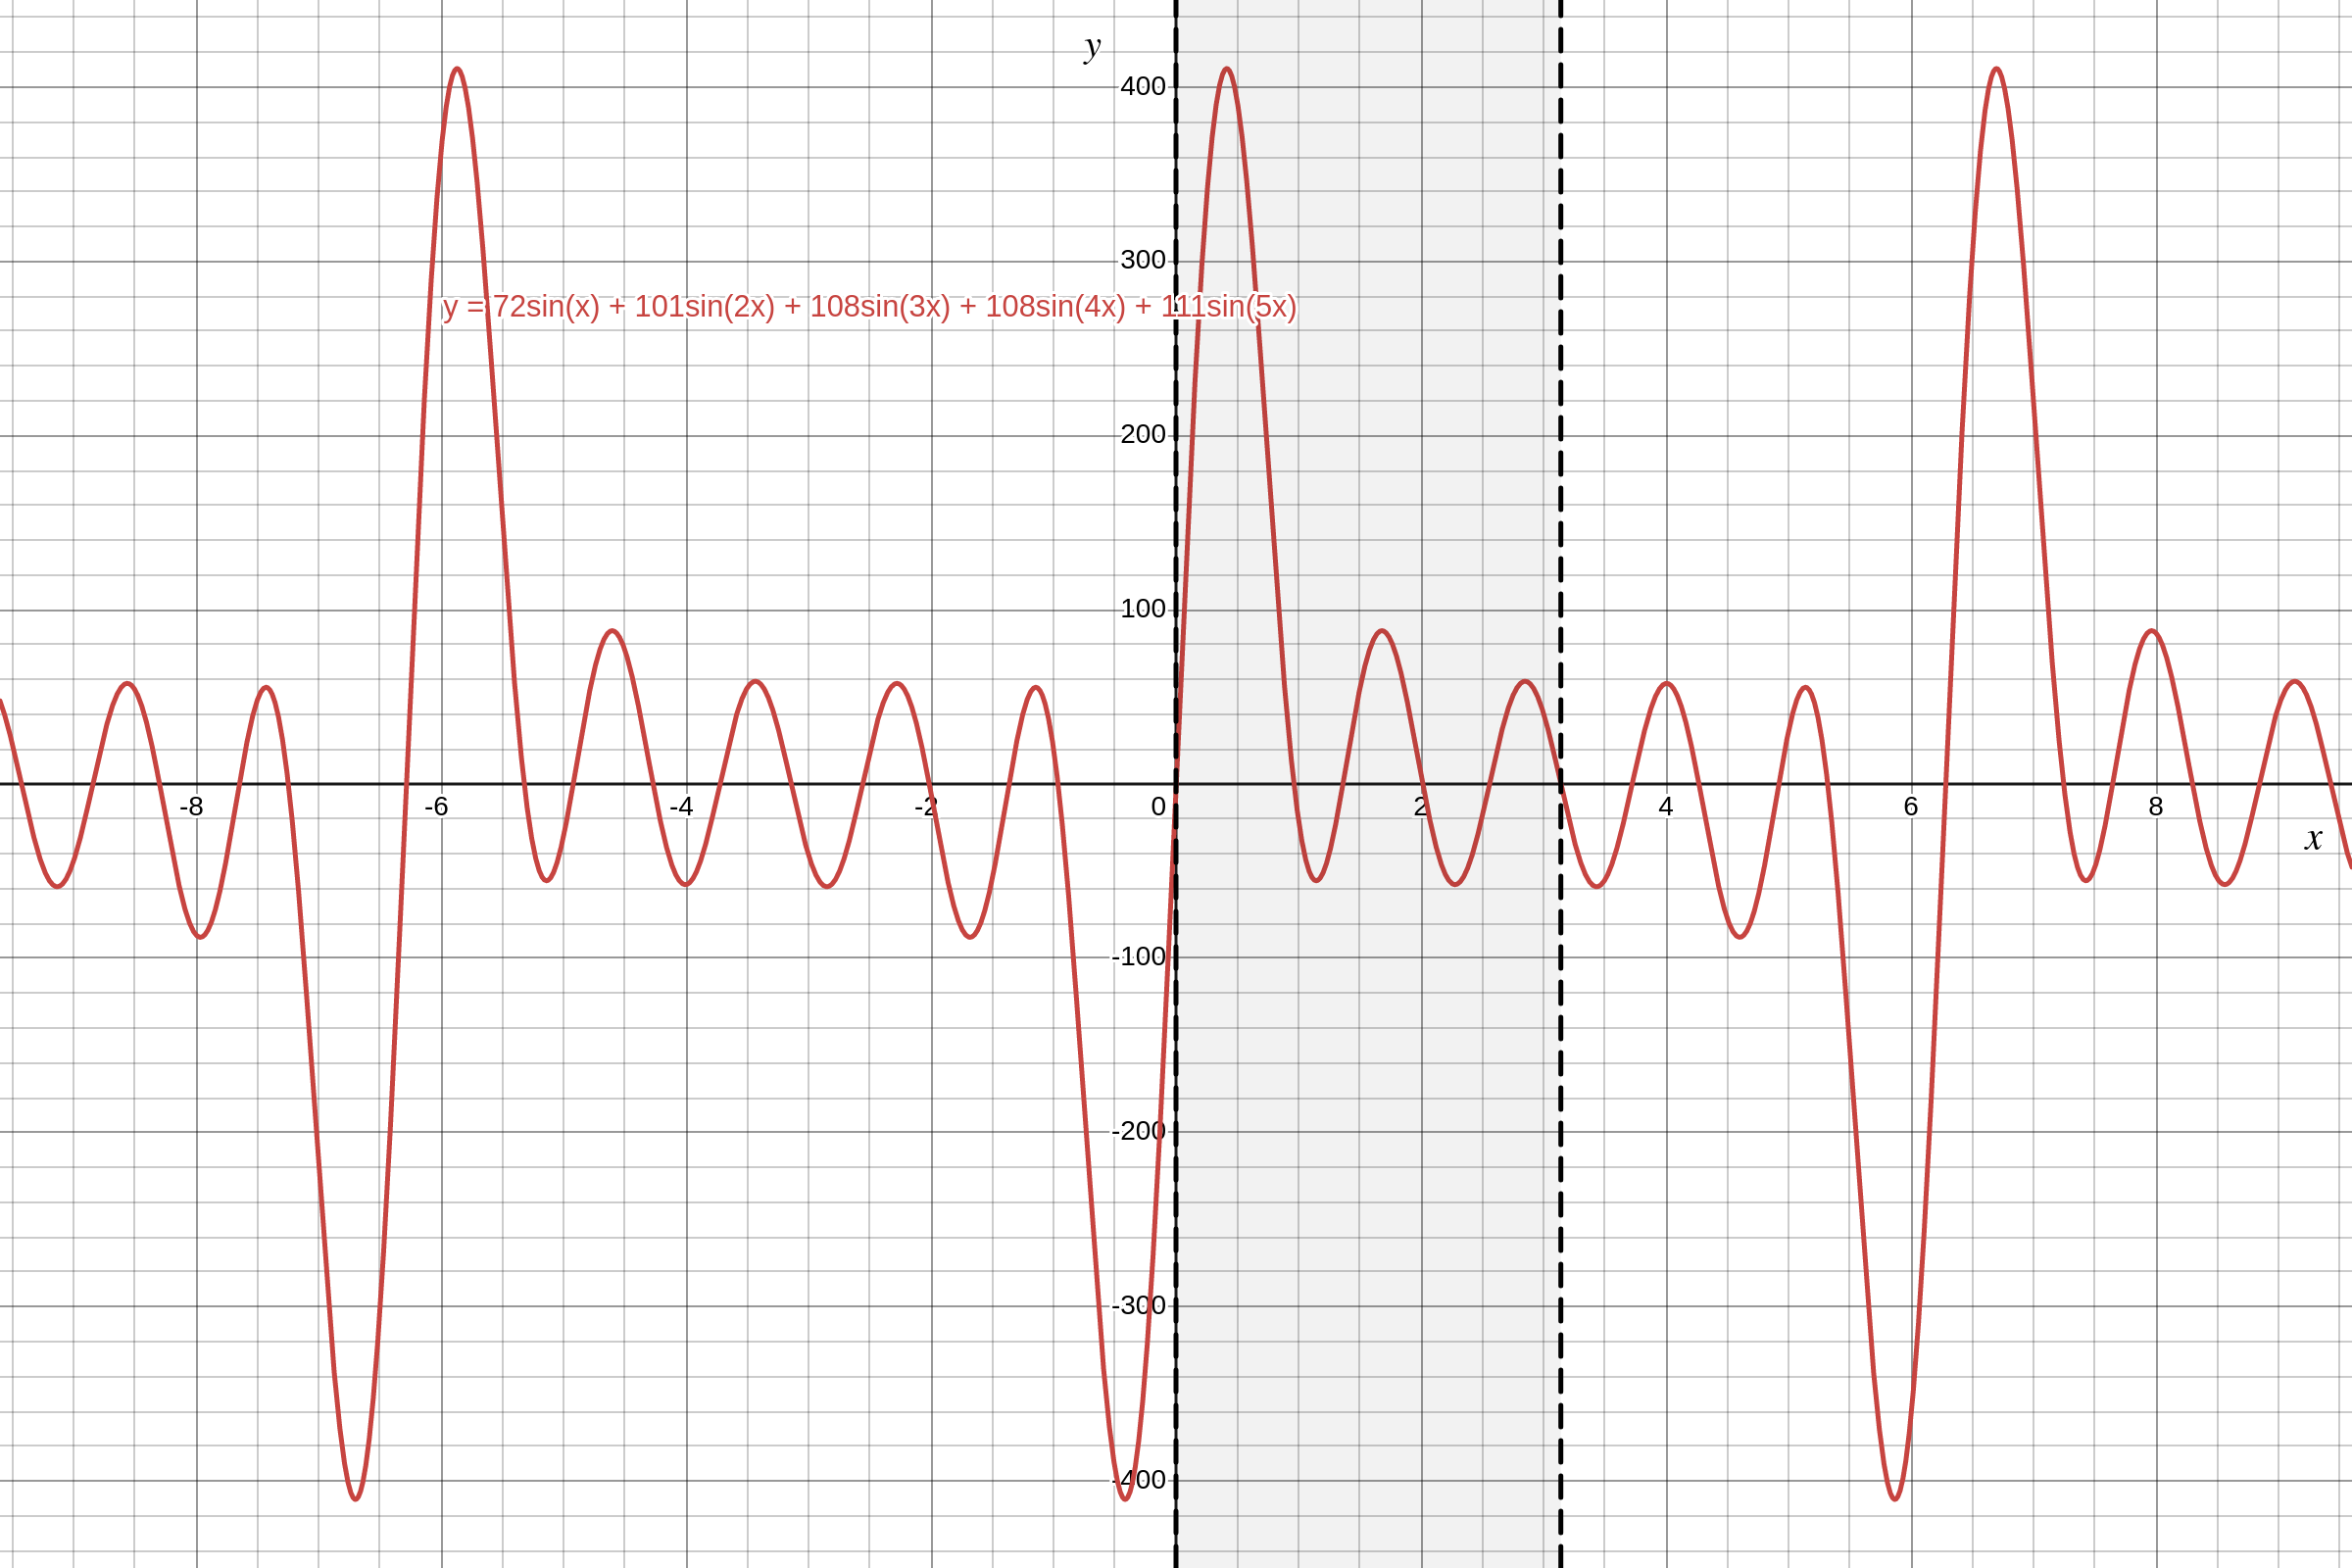
\includegraphics[scale=0.12]{hello-smooth.png}
\caption{This function says ``Hello''}
\label{fig:hellosmooth}
\end{figure}
The coefficients $(72,101,108,108,111)$ are the numbers 
for the characters 
(``\texttt{H}'',``\texttt{e}'',``\texttt{l}'',``\texttt{l}'',``\texttt{o}'')
used in computer systems worldwide (UTF-8).
This assignment will guide you through the integrations needed 
to reveal short messages encoded in functions like this one,
using only the information in their graphs.

\medskip\noindent\textbf{Notation.}
The five sinusoids combined to produce Figure~\ref{fig:hellosmooth}
are plotted in Figure~\ref{fig:FSSbasis}.
Each one is odd and $2\pi$-periodic,
and these two properties are inherited by 
the function in Figure~\ref{fig:hellosmooth}.
For this reason, 
that entire graph can be reconstructed from
the shaded segment, where $0\le x\le \pi$.
We will focus on just this interval in all that follows.
(This explains the choice of axes in Figure~\ref{fig:FSSbasis}.)


\begin{figure}[!ht]
\centering
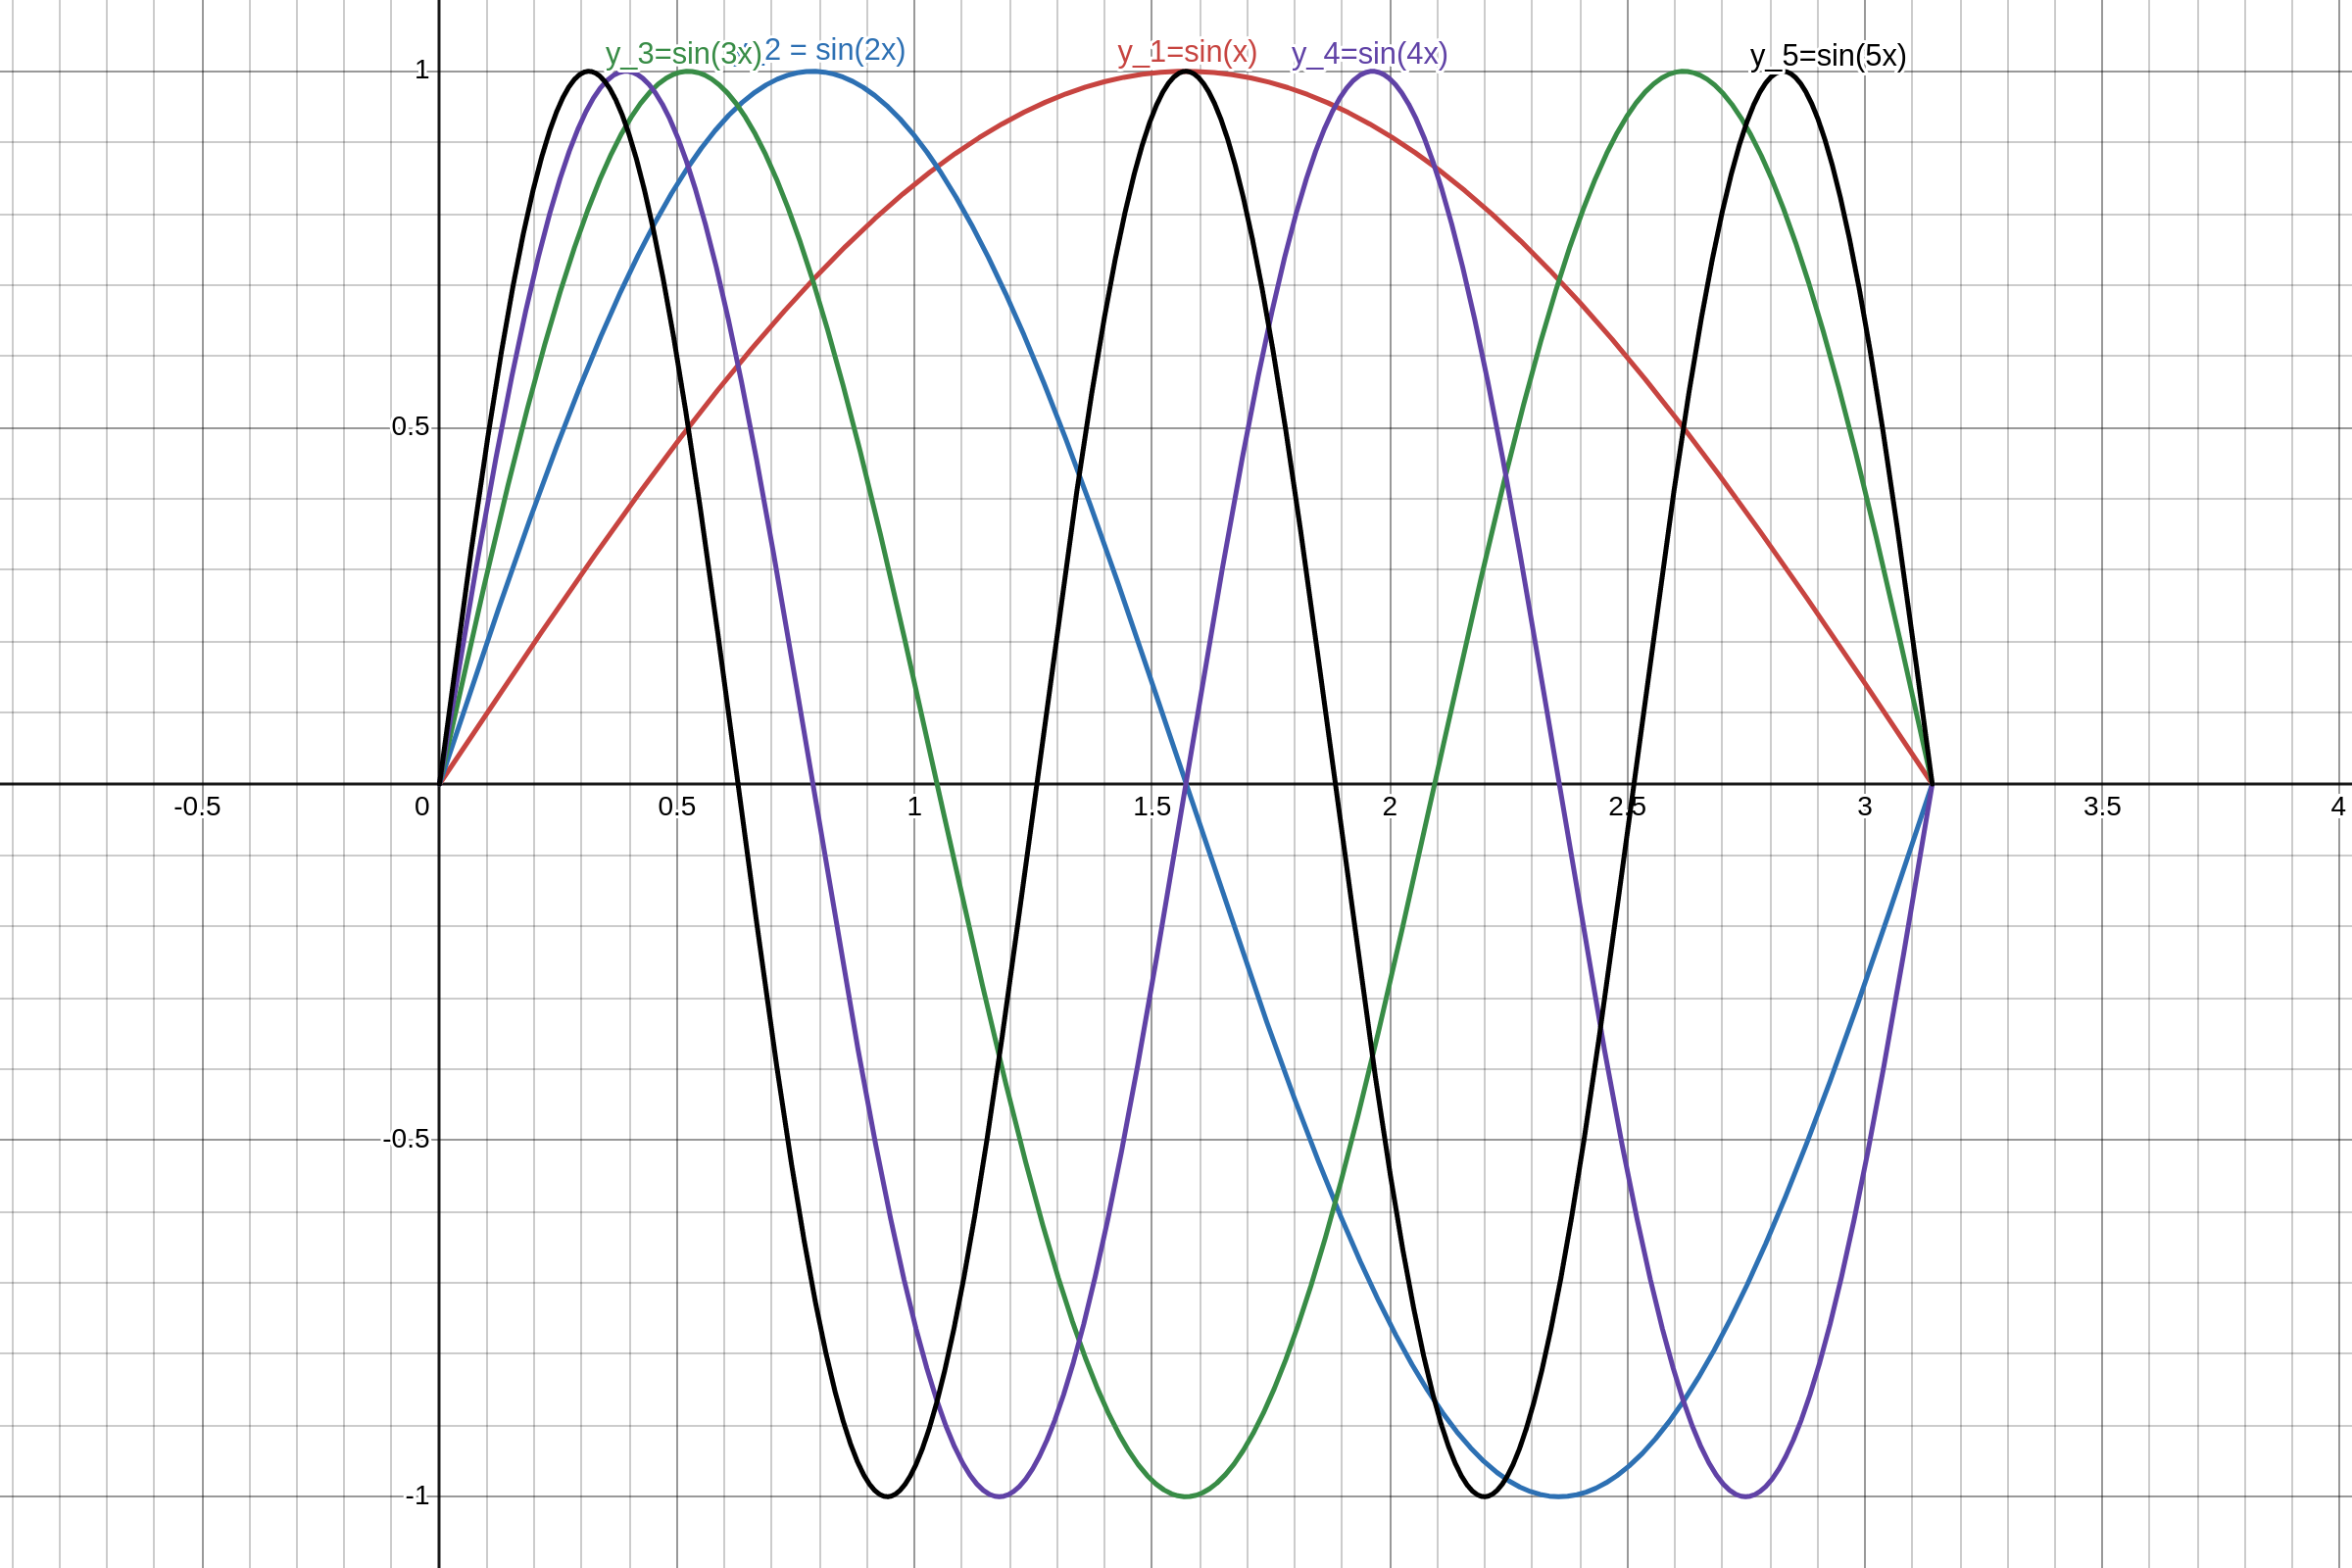
\includegraphics[scale=0.12]{FSS-basis.png}
\caption{Basis functions $y_n=\sin(nx)$ for $n=1,2,3,4,5$}
\label{fig:FSSbasis}
\end{figure}

The sinusoids used in Figures~\ref{fig:hellosmooth} and~\ref{fig:FSSbasis}
are the first five members of the infinite family
\begin{equation}
y_n(x) = \sin(nx),\qquad n=1,2,3,\ldots.
\label{eq:basisdef}
\end{equation}
This assignment concerns various functions of the form exemplified above:
\begin{equation}
f(x) 
= b_1\sin(x) + b_2\sin(2x) + \ldots
= \sum_{k=1}^\infty b_k\sin(kx).
\label{eq:FSS}\end{equation}
Each of these is called a \emph{Fourier Sine Series};
the real-valued constants $b_1,b_2,\ldots$ are called
the \emph{coefficients}.
Later in MATH~101 we will develop a general theory for
``infinite sums'' (officially, \emph{series}).
For this assignment, 
the informal and intuitive approach of treating them
just like ordinary finite sums will suffice.

\goodbreak

\begin{questions}\setcounter{question}{1} 

\question
Use the definitions in line~(\ref{eq:basisdef}) to complete the following.

\begin{parts}
\part[1]\label{testlabel}\starscore14
For arbitrary constants $K,D,m,n$, calculate
\[
\frac{d\ }{dx}\lr[]{K\sin(mx)\cos(nx) + D\cos(mx)\sin(nx) \vphantom{\int}}.
\]
Then use wise choices of $K$ and $D$ 
to find the following indefinite integral,
assuming $m^2\ne n^2$:
\[
\int \sin(mx)\sin(nx)\,dx.
\]

\begin{solution}
    Taking the derivative,
    \begin{align*}
        & \frac{\mathrm d}{\mathrm dx} [K\sin(mx)\cos(nx) + D\cos(mx)\sin(nx)] \\
        = ~& Km \cos(mx) \cos(nx) - Kn \sin(mx)\sin(nx) - Dm \sin(mx) \sin(nx) + Dn \cos(mx) \cos(nx) \\
        = ~& -(Kn + Dm) \sin(mx)\sin(nx) + (Km + Dn) \cos(mx) \cos(nx).
    \end{align*}
    Take $K = n, D = -m$. It then follows that,
    \[ -(Kn + Dm) \sin(mx)\sin(nx) + (Km + Dn) \cos(mx) \cos(nx) = -(n^2 -m^2) \sin(mx) \sin(nx). \]
    Which implies,
    \[ -(n^2 -m^2) \sin(mx) \sin(nx) = \frac{\mathrm d}{\mathrm dx} [n \sin(mx) \cos(nx) - m \cos(mx) \sin(nx)]. \]
    Rearranging and integrating and using our assumption that $n^2 \neq m^2$ we find,
    \[ \int \sin(mx) \sin(nx) \mathrm dx = -\frac{1}{n^2 - m^2} \int \frac{\mathrm d}{\mathrm dx} [n \sin(mx) \cos(nx) - m \cos(mx) \sin(nx)] \mathrm dx. \]
    Applying FTC1, we arrive at,
    \[ \int \sin(mx)\sin(nx) \mathrm dx = \frac{m\cos(mx)\sin(nx) - n\sin(mx)\cos(nx)}{n^2 - m^2} + C. \]
    
\end{solution}

\part[1]\label{stepfunction}\starscore14
Determine the constant $R$ 
that makes the following equation valid
for all positive integers $m$ and $n$.
Explain why the stated equation holds.
\[
\int_0^\pi \sin(mx) \sin(nx)\,dx 
= \begin{cases}
0, &\text{if}\ m\ne n,
\\
R, &\text{if}\ m=n.
\end{cases}\]

\begin{solution}
    Assume $m = n$ and $m, n \in \mathbb{Z}^+$. In our integral, we substitute $u = nx$, and apply the identity $\sin(x)^2 = \frac{1}{2}(1 - \sin(2x))$.

    \[ \int^{\pi}_{0} \sin(mx)\sin(nx) = \int^{\pi}_{0} \sin(nx)^2 \mathrm dx = \frac{1}{2n} \left( u - \frac{1}{2}\sin(2u) \right) \Big|^{n\pi}_{0} = \frac{\pi}{2}\]

    This must be our value for $R$.
    
    Assume $m, n \in \mathbb{Z}^+$ and $m \neq n$.

    Note that our assumption in (\ref{testlabel}) that $m^2 \neq n^2$ implies $n \neq m$.

    By FTC2,

    \begin{align*}
        &\int^{\pi}_{0} \sin(mx)\sin(nx) \mathrm dx \\
        = ~& \frac{m\cos(m\pi)\sin(n\pi) - n\sin(m\pi)\cos(n\pi)}{n^2 - m^2} - \frac{m\cos(0)\sin(0) - n\sin(0)\cos(0)}{n^2 - m^2} \\
        \intertext{As $\sin(n\pi) = 0$ for any $n \in \mathbb{Z}^+$, and $\sin(0) = 0$, the top of each fraction is $0$, so,}
        = ~& 0
    \end{align*}
\end{solution}

\begin{EnvUplevel}
For any given function $f(x)$ integrable on $[0,\pi]$,
we now use the constant $R$ found above to define
\begin{equation}
B_k(f) = \frac{1}{R}\int_0^\pi f(x)\sin(k x)\,dx,
\qquad k=1,2,3,\ldots.
\label{eq:FSSBk}
\end{equation}
\end{EnvUplevel}


\part[1]\starscore14
Consider the specific function plotted in Figure~\ref{fig:hellosmooth}, namely,
\[
f(x) = 72\sin(x) + 101\sin(2x) + 108\sin(3x) + 108\sin(4x) + 111\sin(5x).
\]
Calculate $B_n(f)$ for each integer $n\ge1$.

\begin{solution}
    Using $R = \frac{\pi}{2}$ the formula for $B_k$ on $f$ for some arbitrary integer $n \geq 1$,
    \begin{align*}
        B_n = & \frac{2}{\pi} \int^{\pi}_{0} 72\sin(x) \sin(nx) + 101\sin(2x) \sin(nx) \\
        & + 108\sin(3x) \sin(nx) + 108\sin(4x) \sin(nx) + 111\sin(5x) \sin(nx) \mathrm dx \\
        \intertext{Applying the linearity of integrals,}
        = & \frac{2}{\pi} \Big(
            72 \int^{\pi}_{0} \sin(x)\sin(nx) + 101 \int^{\pi}_{0} \sin(2x)\sin(nx) \\
        & + 108 \int^{\pi}_{0} \sin(3x) \sin(nx) \mathrm dx + 108 \int^{\pi}_{0} \sin(4x)\sin(nx) \mathrm dx + 111 \int^{\pi}_{0} \sin(5x)\sin(nx) \mathrm dx \Big)
    \end{align*}

    By (\ref{stepfunction}) when $n = 1$, $\sin(nx) = \sin(x)$, all integrals except $\int^{\pi}_{0} \sin(x)\sin(x) \mathrm dx$ equal 0. So therefore we have $B_1 = \frac{2}{\pi}\left( 72 \times  \frac{\pi}{2} \right) = 72$.

    When $n = 2$, $\sin(nx) = \sin(2x)$, all integrals except $\int^{\pi}_{0} \sin(2x)\sin(2x) \mathrm dx$ equal 0. Therefore, we have $B_2 = \frac{2}{\pi} \left( 101 \times \frac{\pi}{2} \right) = 101$.

    When $n = 3$, $\sin(nx) = \sin(3x)$, all integrals except $\int^{\pi}_{0} \sin(3x)\sin(3x) \mathrm dx$ equal 0. Therefore, we have $B_3 = \frac{2}{\pi} \left( 108 \times \frac{\pi}{2} \right) = 108$.

    When $n = 4$, $\sin(nx) = \sin(4x)$, all integrals except $\int^{\pi}_{0} \sin(4x)\sin(4x) \mathrm dx$ equal 0. Therefore, we have $B_4 = \frac{2}{\pi} \left( 108 \times \frac{\pi}{2} \right) = 108$.

    When $n = 5$, $\sin(nx) = \sin(5x)$, all integrals except $\int^{\pi}_{0} \sin(5x)\sin(5x) \mathrm dx$ equal 0. Therefore, we have $B_5 = \frac{2}{\pi} \left( 111 \times \frac{\pi}{2} \right) = 111$.
\end{solution}

\part[1]\starscore14
Now think about a general function $f$ with the form shown below,
where each $b_k$ is a constant:
\[
f(x) = b_1\sin(x) + b_2\sin(2x) + \ldots
= \sum_{k=1}^\infty b_k\sin(kx).
\]
Find a formula that expresses $b_n$ in terms of one or more of the numbers
$B_k(f)$ defined in line~(\ref{eq:FSSBk}).
Your result should be valid for every integer $n\ge1$.
Explain why your formula holds.

\begin{solution}
    Assume $n \geq 1$.
    
    Let us apply $B_n$ on $f$. Then we have:

    \[ B_n(f) = \frac{2}{\pi} \int^{\pi}_{0} \sum^{\infty}_{k = 1} [b_k \sin(kx)]  \sin(nx) \mathrm dx. \]
    
    Consider the $n^\text{th}$ term in the series $\sum^{\infty}_{k = 1} b_k \sin(kx)$. That is the only term that satisfies the property that $k = n$, by (\ref{stepfunction}), all the other terms in that series vanish to zero. Again by (\ref{stepfunction}), we know that the value of that $n^\text{th}$ term is $R = \frac{\pi}{2}$. This means $B_n(f) = \frac{2}{\pi} \int^{\pi}_{0} \sum^{\infty}_{0} b_k \sin(kx) \sin(nx) \mathrm dx = \frac{2}{\pi} \int^{\pi}_{0} b_n \sin(nx) \sin(nx) \mathrm dx$. Reapplying (\ref{stepfunction}) and the linearity of integrals for the final time, we arrive at $B_n(f) = \frac{2}{\pi} b_n \frac{\pi}{2} = b_n$.

\end{solution}

\end{parts}



\begin{EnvUplevel}
For smooth periodic functions like the one graphed in Figure~\ref{fig:hellosmooth},
the integrals shown in line~(\ref{eq:FSSBk}) are excellent candidates 
for approximate evaluation by the Trapezoidal Rule.
Specialized analysis reveals that the actual difference 
between the exact value  and its Trapezoidal approximation is much,
much smaller than the standard estimate shown in class suggests.
So we choose the Trapezoidal Rule for all of our integral approximations below.
\end{EnvUplevel}

\question
Imagine dividing $[0,\pi]$ into $N=8$ subintervals, with endpoints 
\[
x_0 = 0,\ x_1=\frac{\pi}8,\ \ldots,\ x_i = \frac{i\pi}{8},\ \ldots,\ x_8 = \frac{8\pi}8,
\]
and evaluating the numbers $f_i = f(x_i)$ for $i=0,1,\ldots,8$.
For $f(x)$ as shown in Figure~\ref{fig:hellosmooth}, the  $9$ numbers $f_i$, in order, are approximately
\[
0.0,\ 
409.3,\ 
149.8,\ 
-53.9,\ 
75.0,\ 
19.3,\ 
-52.2,\ 
50.5,\ 
0.0.
\]
\begin{parts}
\part[1]\starscore24
Use all of these values to calculate Trapezoidal-rule approximations
for the integrals $B_1(f),\ldots,B_5(f)$.
(Call these $B_n^{\rm trap}(f)$.)
Report each answer with 3 decimal places.

\begin{solution}
Using this Python script,
    \begin{verbatim}
from math import pi, sin

R = pi / 2


def tr_rule(values: list[float], dx: float, n: int) -> float:
    assert len(values) == 9
    x_k = [dx * i for i in range(9)]
    return (1 / R) * (dx * (1/2 * values[0] * sin(n * x_k[0])
                            + sum([values[i] * sin(n * x_k[i])
                                  for i in range(1, 8)])
                            + 1/2 * values[8] * sin(n * x_k[8])))


f_k: list[float] = [0.0, 409.3, 149.8, -53.9, 75.0, 19.3, -52.2, 50.5, 0.0]

for i in range(1, 6):
    print(f"B_{i}(f) = {round(tr_rule(f_k, pi / 8, i), 3)}")
    \end{verbatim}

We find that:

\begin{itemize}
    \item $B^{\text{trap}}_1(f) = 72.001$
    \item $B_2^{\text{trap}}(f) = 100.987$
    \item $B_3^{\text{trap}}(f) = 108.014$
    \item $B^{\text{trap}}_4(f) = 108.000$
    \item $B^{\text{trap}}_5(f) = 111.007$
\end{itemize}
\end{solution}

\part[1]\starscore14
Report, to 3 significant digits,
the 5 numbers $B_n^{\rm trap}(f)-B_n(f)$,
$n=1,\ldots,5$.

\begin{solution}
    Some simple subtraction yields:
    \begin{itemize}
        \item $B^{\text{trap}}_1(f) - B_1 = 72.001 - 72 = 0.001$
        \item $B_2^{\text{trap}}(f) - B_2 = 100.987 - 101 = -0.013$
        \item $B_3^{\text{trap}}(f) - B_3 = 108.014 - 108 = 0.014$
        \item $B^{\text{trap}}_4(f) - B_4 = 108.000 - 108 = 0.000$
        \item $B^{\text{trap}}_5(f) - B_5 = 111.007 - 111 = 0.007$
    \end{itemize}
\end{solution}

\end{parts}

Your writeup for this problem should describe your method 
for computing the numbers $B_n^{\rm trap}(f)$
in enough detail that a patient reader could reproduce your work.
Show documentation appropriate for whatever approach you used:
a code listing (any language is acceptable), 
a spreadsheet sample,
or selected screenshots, etc.

\begin{EnvUplevel}
The next question applies the ideas from Question~3 at scale.
It involves rather large numbers $N$ and $R$, 
so computer assistance in evaluating
the individual Trapezoidal-Rule approximations will be essential.
You will need to apply the Trapezoidal Rule to $R+1$ different integrals,
so a systematic computer-assisted approach is recommended also for this.
\end{EnvUplevel}

\question
A special message for the students in your small class section
has been UTF-8 encoded in a list of positive integers $b_1,b_2,\ldots,b_R$.
These numbers provide the coefficients that define a new function
\[
f(x) = b_1\sin(x) + b_2\sin(2x) + \ldots + b_R \sin(Rx).
\]
\begin{parts}
\part
Acquire the list of numbers $f_i$, $i=0,\ldots,N$,
specific to your small class.
These are available on Canvas, in an appropriately-named \texttt{CSV} file.
The given numbers are approximate values $f_i\approx f(x_i)$,\
where
$x_i = \frac{i\pi}{N}$, $i=0,1,2,\ldots,N$.
(There is nothing to hand in for this part.)
\part[1]\starscore14
Determine and report your specific value of $N$.
Then produce a computer-generated plot of the curve $y=f(x)$ 
on the interval $0\le x\le\pi$.

\begin{solution}

    Our $N$ was $128$.
    
    \centering
    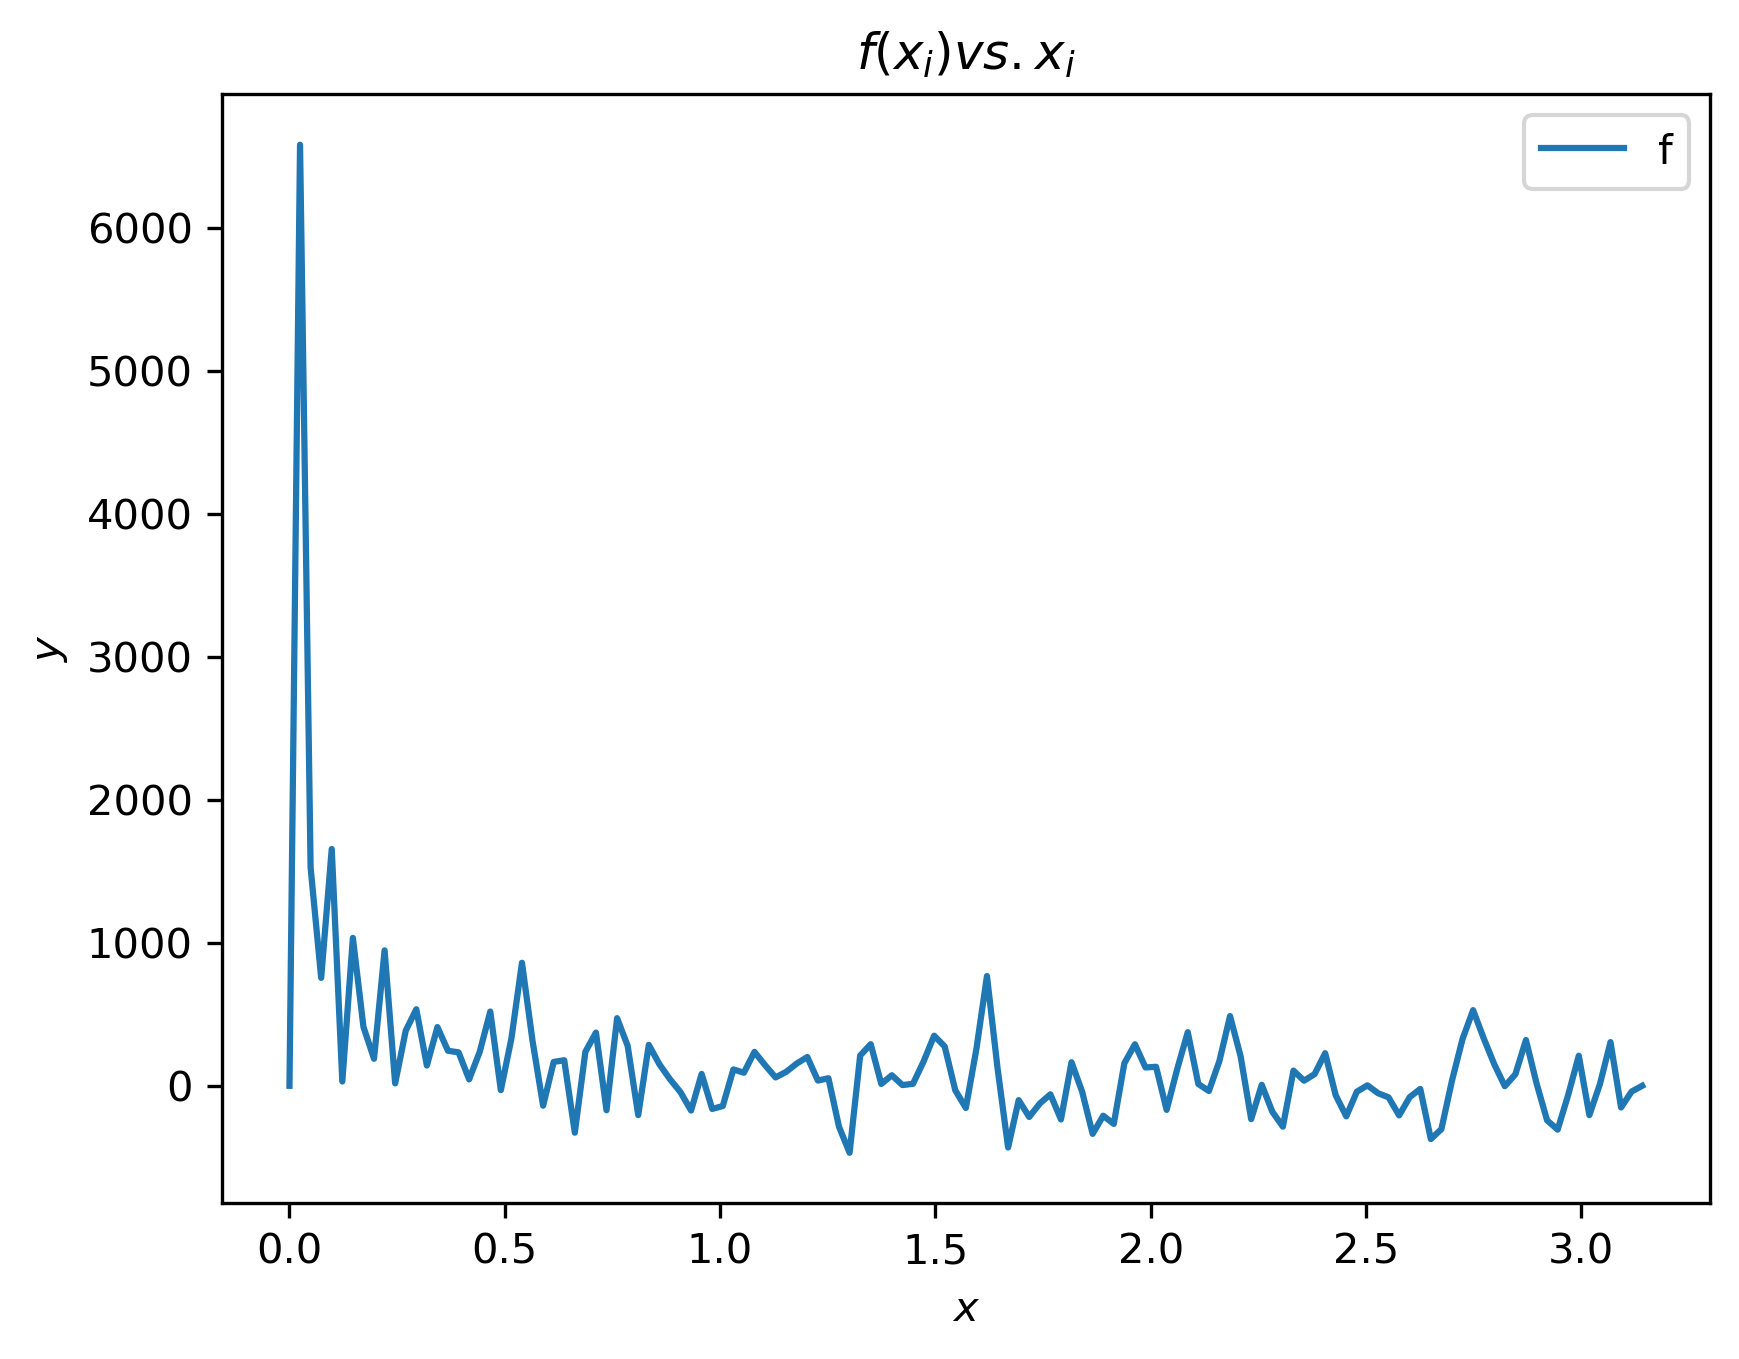
\includegraphics[scale=0.2]{4b_plot.png}  

\end{solution}

\part[5]\starscore34
Use the Trapezoidal Rule to find the number $R$
and the coefficients $b_1,\ldots,b_R,b_{R+1}$.
To recognize $R$, note that $b_1,\ldots,b_R$ are all positive,
whereas $b_{R+1}=0$.
Report the coefficients $b_1,\ldots,b_R$ as a comma-separated
list of positive integers.

Just as in Question~3, your submission should describe your methods
in enough detail that a patient reader could reproduce your work.

\begin{solution}
    Using this Python script:

    \begin{verbatim}
from math import sin, pi
import pandas as pd
import numpy as np

values = pd.read_csv(r"./A17.csv", names=[r"f"])

n = values.iloc[-1].name

dx = pi/n

x_axis = np.arange(0, np.pi + dx, dx)

values['x'] = x_axis


def tr_rule(f: pd.Series, x: pd.Series, dx: float, R: int):
    return (
        (2 / pi) * dx * (
            (1/2 * f.iloc[0] * sin(R * x.iloc[0])) +
            sum(f.iloc[1:-1] * (x.iloc[1:-1] * R).map(sin)) +
            (1/2 * f.iloc[-1] * sin(R * x.iloc[-1]))
        )
    )


b_k_raw: list[float] = []

last_result = float('inf')
i = 1
while round(last_result, 6) > 0:
    last_result = tr_rule(values['f'], values['x'], dx, i)
    b_k_raw.append(last_result)
    i += 1

b_k = list(filter(lambda x: x != 0, [round(b_i) for b_i in b_k_raw]))

print(b_k)

resulting_chars = [chr(b_i) for b_i in b_k]

print("".join(resulting_chars))
    \end{verbatim}
    
    The values for $b_1 ... b_R$ are (note $R = 101$):

    83, 99, 105, 101, 110, 99, 101, 32, 105, 115, 32, 110, 111, 116, 32, 111, 110, 108, 121, 32, 97, 32, 100, 105, 115, 99, 105, 112, 108, 101, 32, 111, 102, 32, 114, 101, 97, 115, 111, 110, 32, 98, 117, 116, 32, 97, 108, 115, 111, 32, 111, 110, 101, 32, 111, 102, 32, 114, 111, 109, 97, 110, 99, 101, 32, 97, 110, 100, 32, 112, 97, 115, 115, 105, 111, 110, 46, 32, 45, 32, 83, 116, 101, 112, 104, 101, 110, 32, 72, 97, 119, 107, 105, 110, 103, 32, 91, 67, 65, 68, 93
\end{solution}

\part[1]\starscore04
Turn the UTF-8 encodings $b_1,\ldots,b_R$ into a readable message
and report it.
This task needs no Calculus,
so you are invited simply to paste your list of numbers from part~(c)
into the online tool linked here:
\url{https://personal.math.ubc.ca/~loew/utf8-to-text.html}.

\begin{solution}
\begin{mdframed}[style=QuoteFrame]
% Delete the quotation here and put yours in its place.
\raggedright\texttt{%
Science is not only a disciple of reason but also one of romance and passion. - Stephen Hawking [CAD]
}
\end{mdframed}

\end{solution}
\end{parts}

\question
The integrals defined in line~(\ref{eq:FSSBk}) are meaningful numbers
for any integrable function $f$.
Treating a given function as if it were a combination of periodic
functions opens the door to \emph{Fourier analysis},
a powerful tool with many applications in science, engineering, and mathematics.
Present exact calculations where they are requested below,
but use suitable software to produce the corresponding plots.

\begin{parts}
\part[1]\starscore14
Let $f(x)=1$ for $0\le x\le\pi$.
Find a formula for $B_n(f)$ valid for every integer $n\ge1$.
\begin{solution}
    \begin{align*}
        B_n(f) &=  \frac{2}{\pi} \int^{\pi}_{0} \sin(nx) \mathrm dx \\
               &= \frac{2}{\pi} \left( -\frac{1}{n} \cos(nx) \Big|^{\pi}_{0} \right) \\
               &= \frac{2}{\pi n}\left( 1 - \cos(n\pi) \right) \\
    \end{align*}

    By the periodicity of $\cos(n\pi)$, when $n$ is even, $\cos(n\pi) = 1$, and when $n$ is odd, $\cos(n\pi) = -1$.

    Therefore, using this property, we can conclude:

    \[
        B_n(f) = 
        \begin{cases}
            0 & \text{if } n ~\text{is even} \\
            \frac{4}{\pi n} & \text{if } n ~\text{is odd}
        \end{cases}
    \]
\end{solution}
\part[1]
Make three plots showing $y=f(x)$ and $y=S_N(x)$ on the same axes, where
\[
S_N(x) = \sum_{n=1}^N B_n(f) \sin(nx).
\]
Use $N=3$ for the first plot, $N=5$ for the second, and $N=11$ for the third.
\begin{solution}

    \centering
    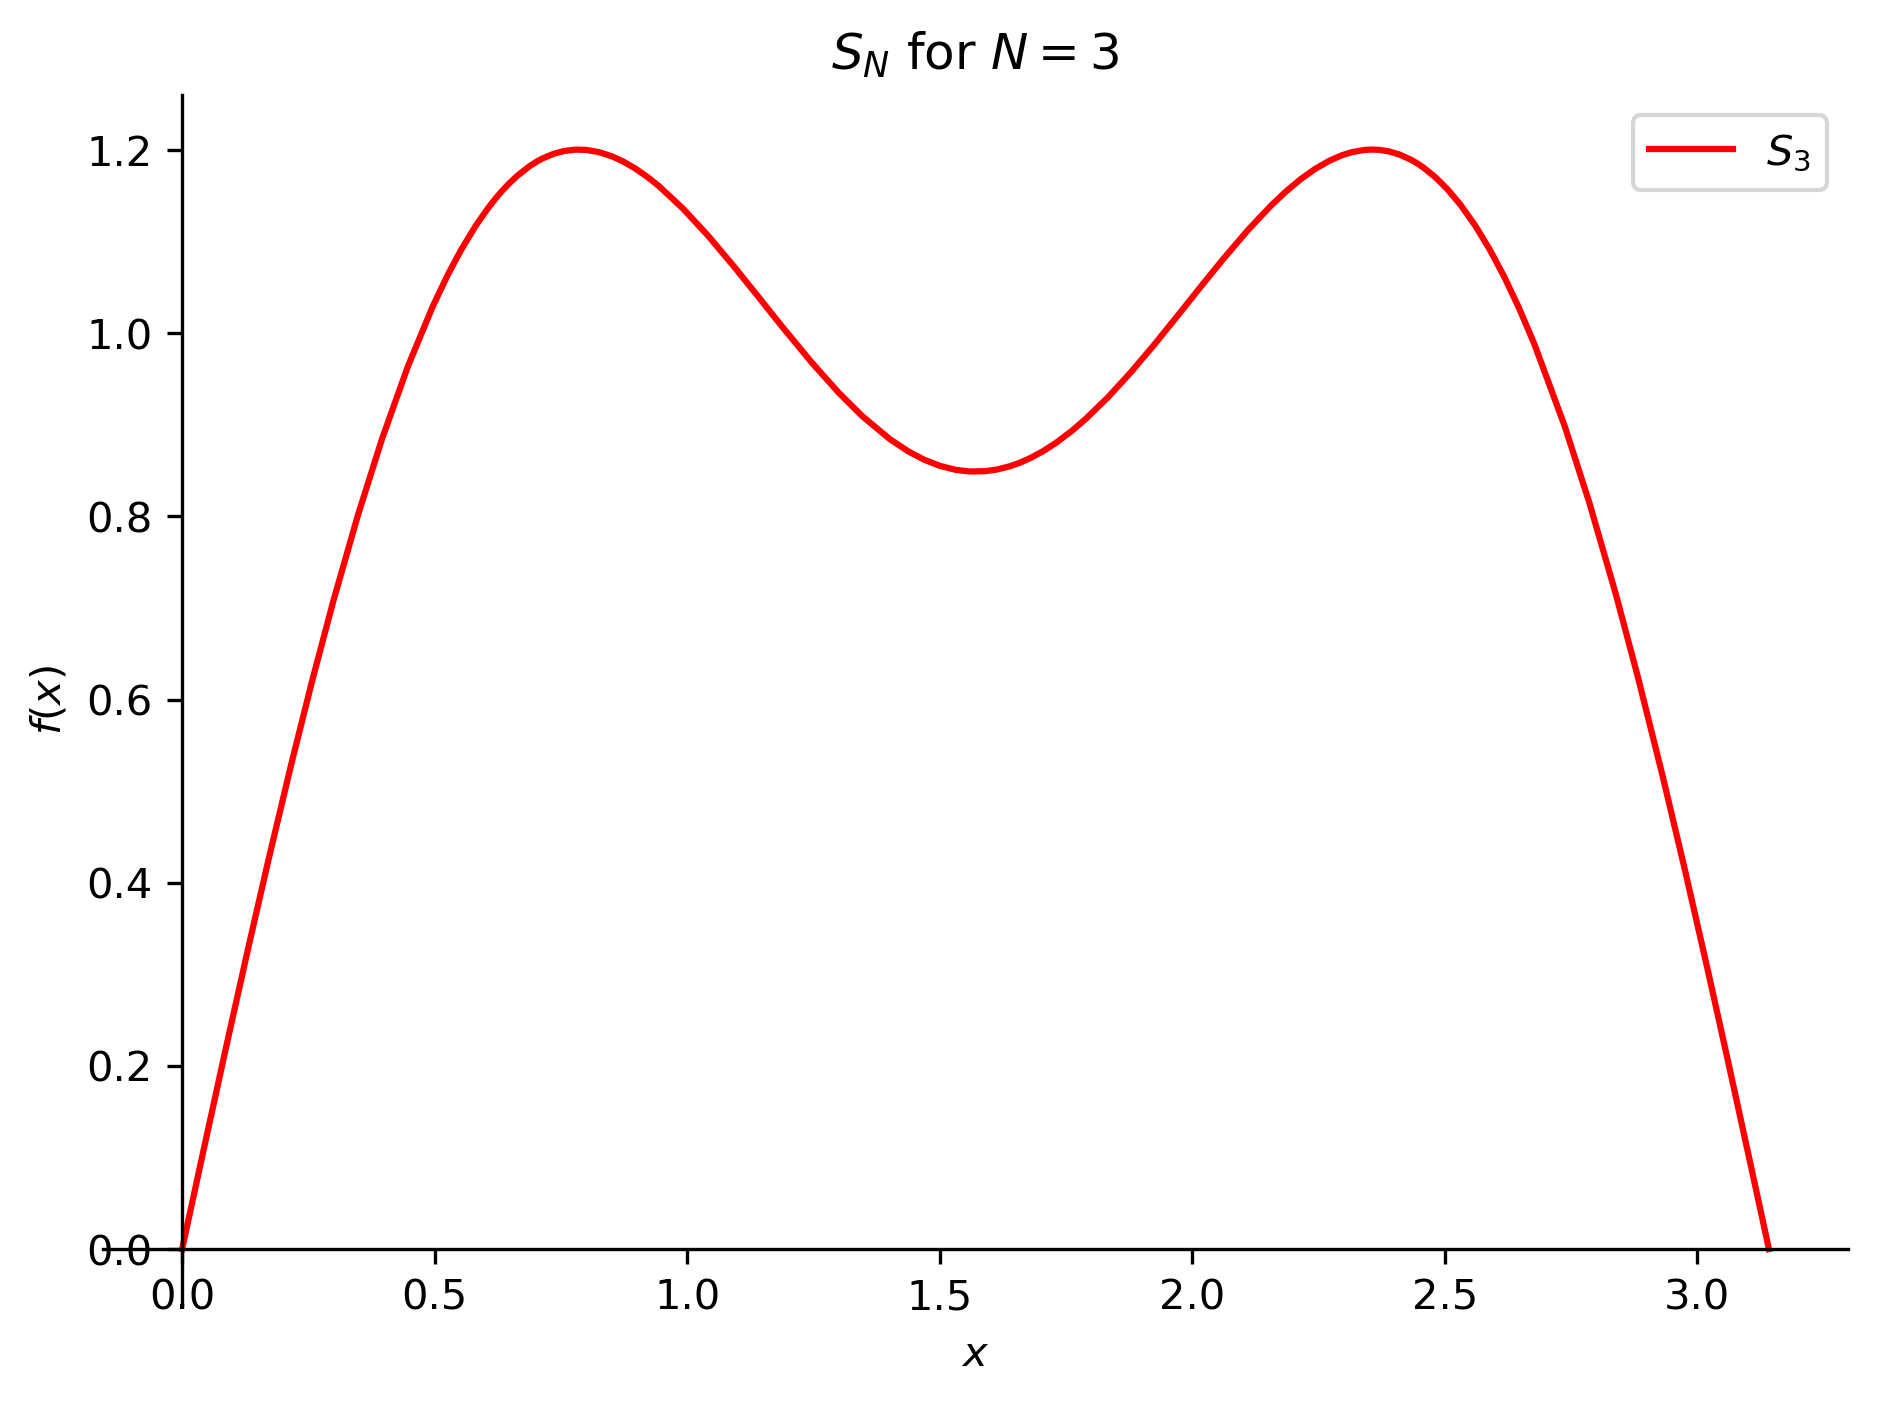
\includegraphics[scale=0.67]{5bs3.png}

    \centering
    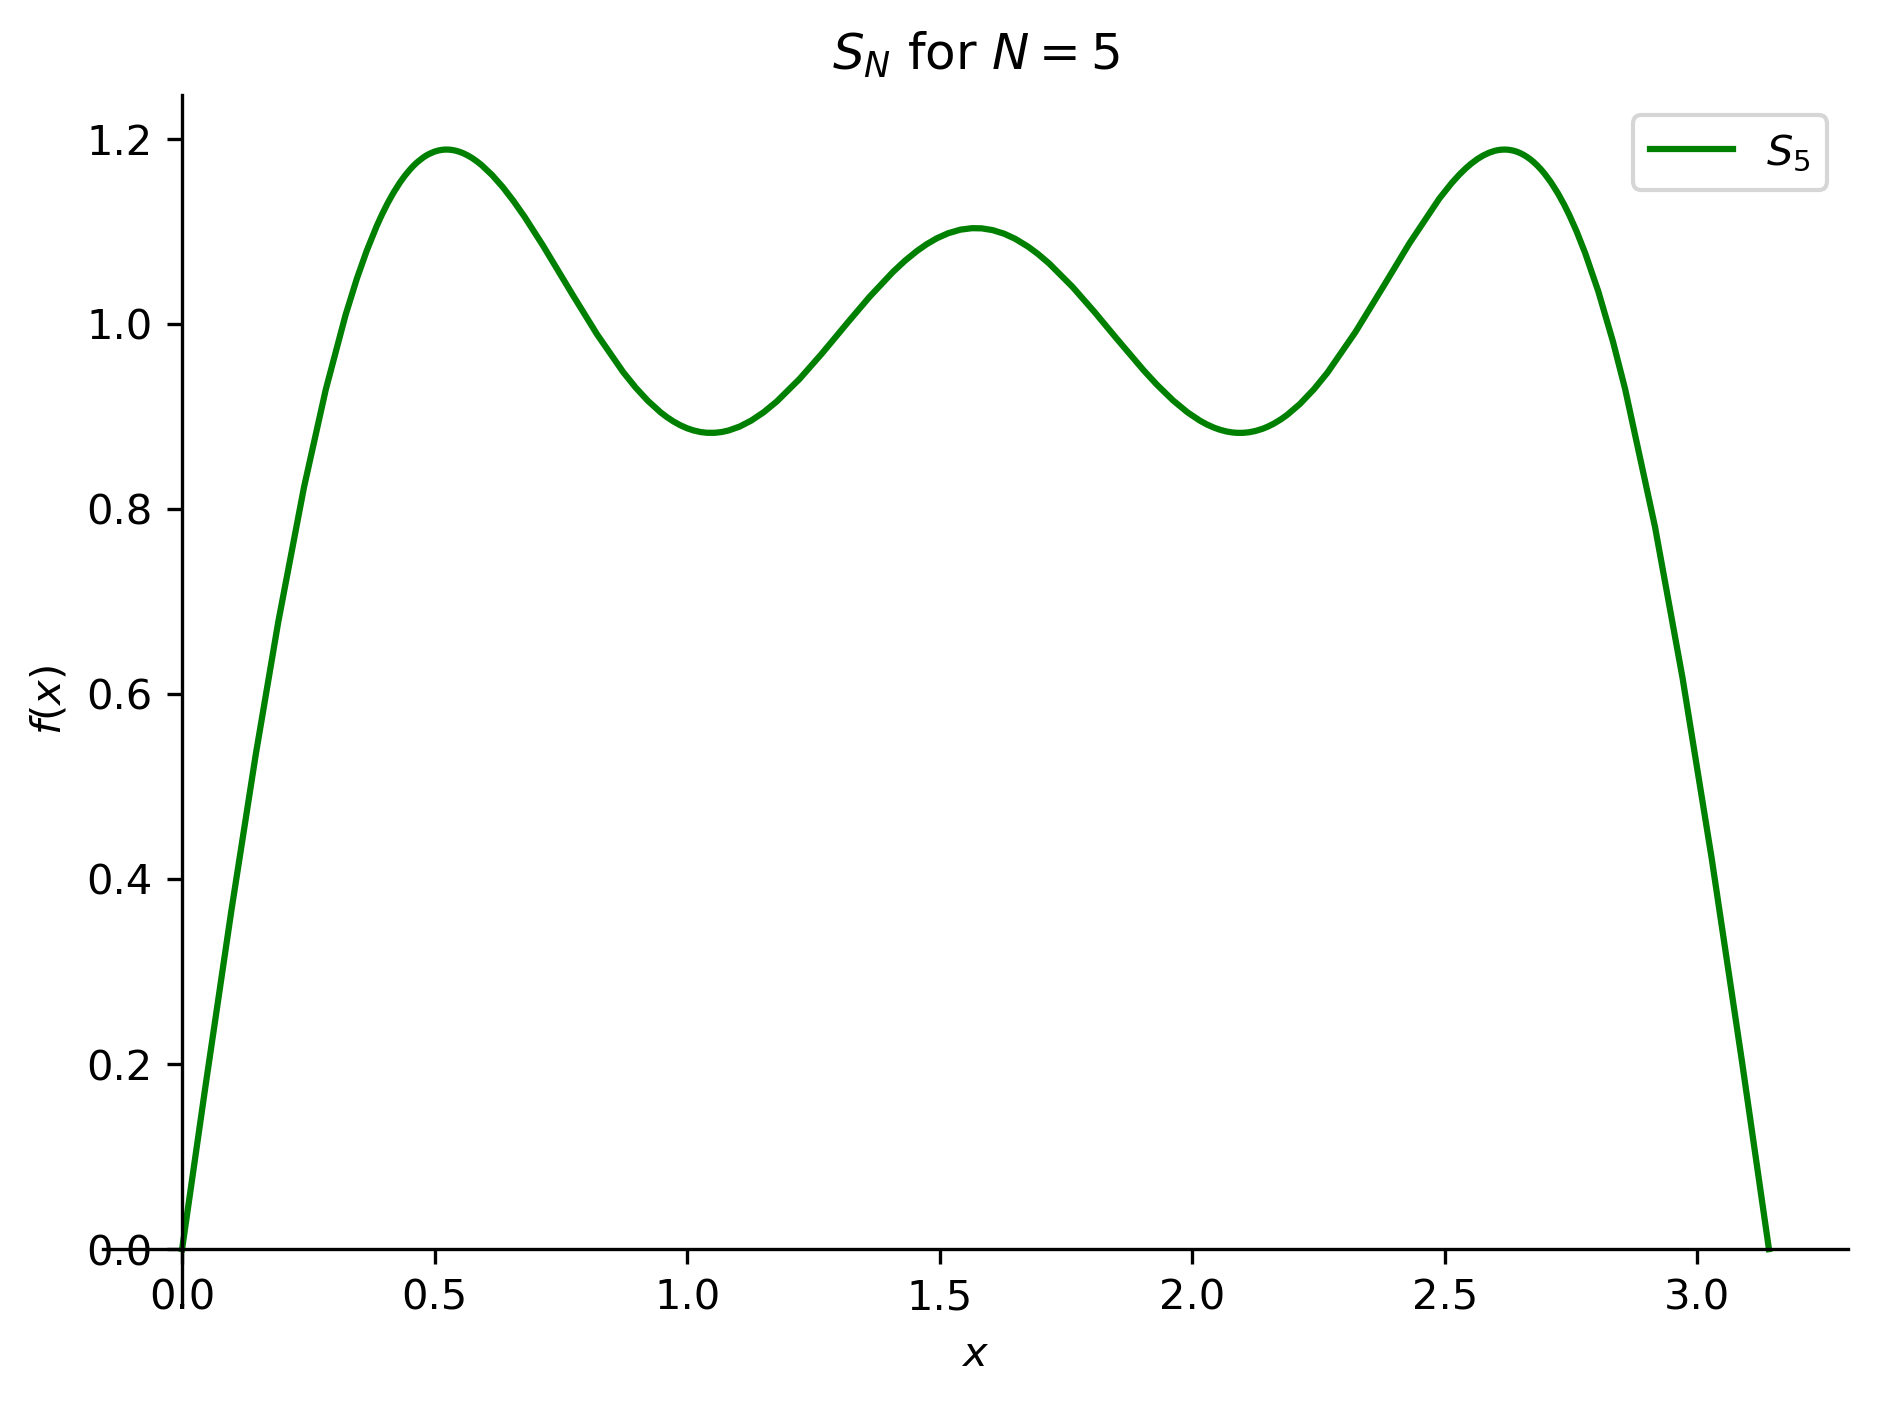
\includegraphics[scale=0.67]{5bs5.png}

    \centering
    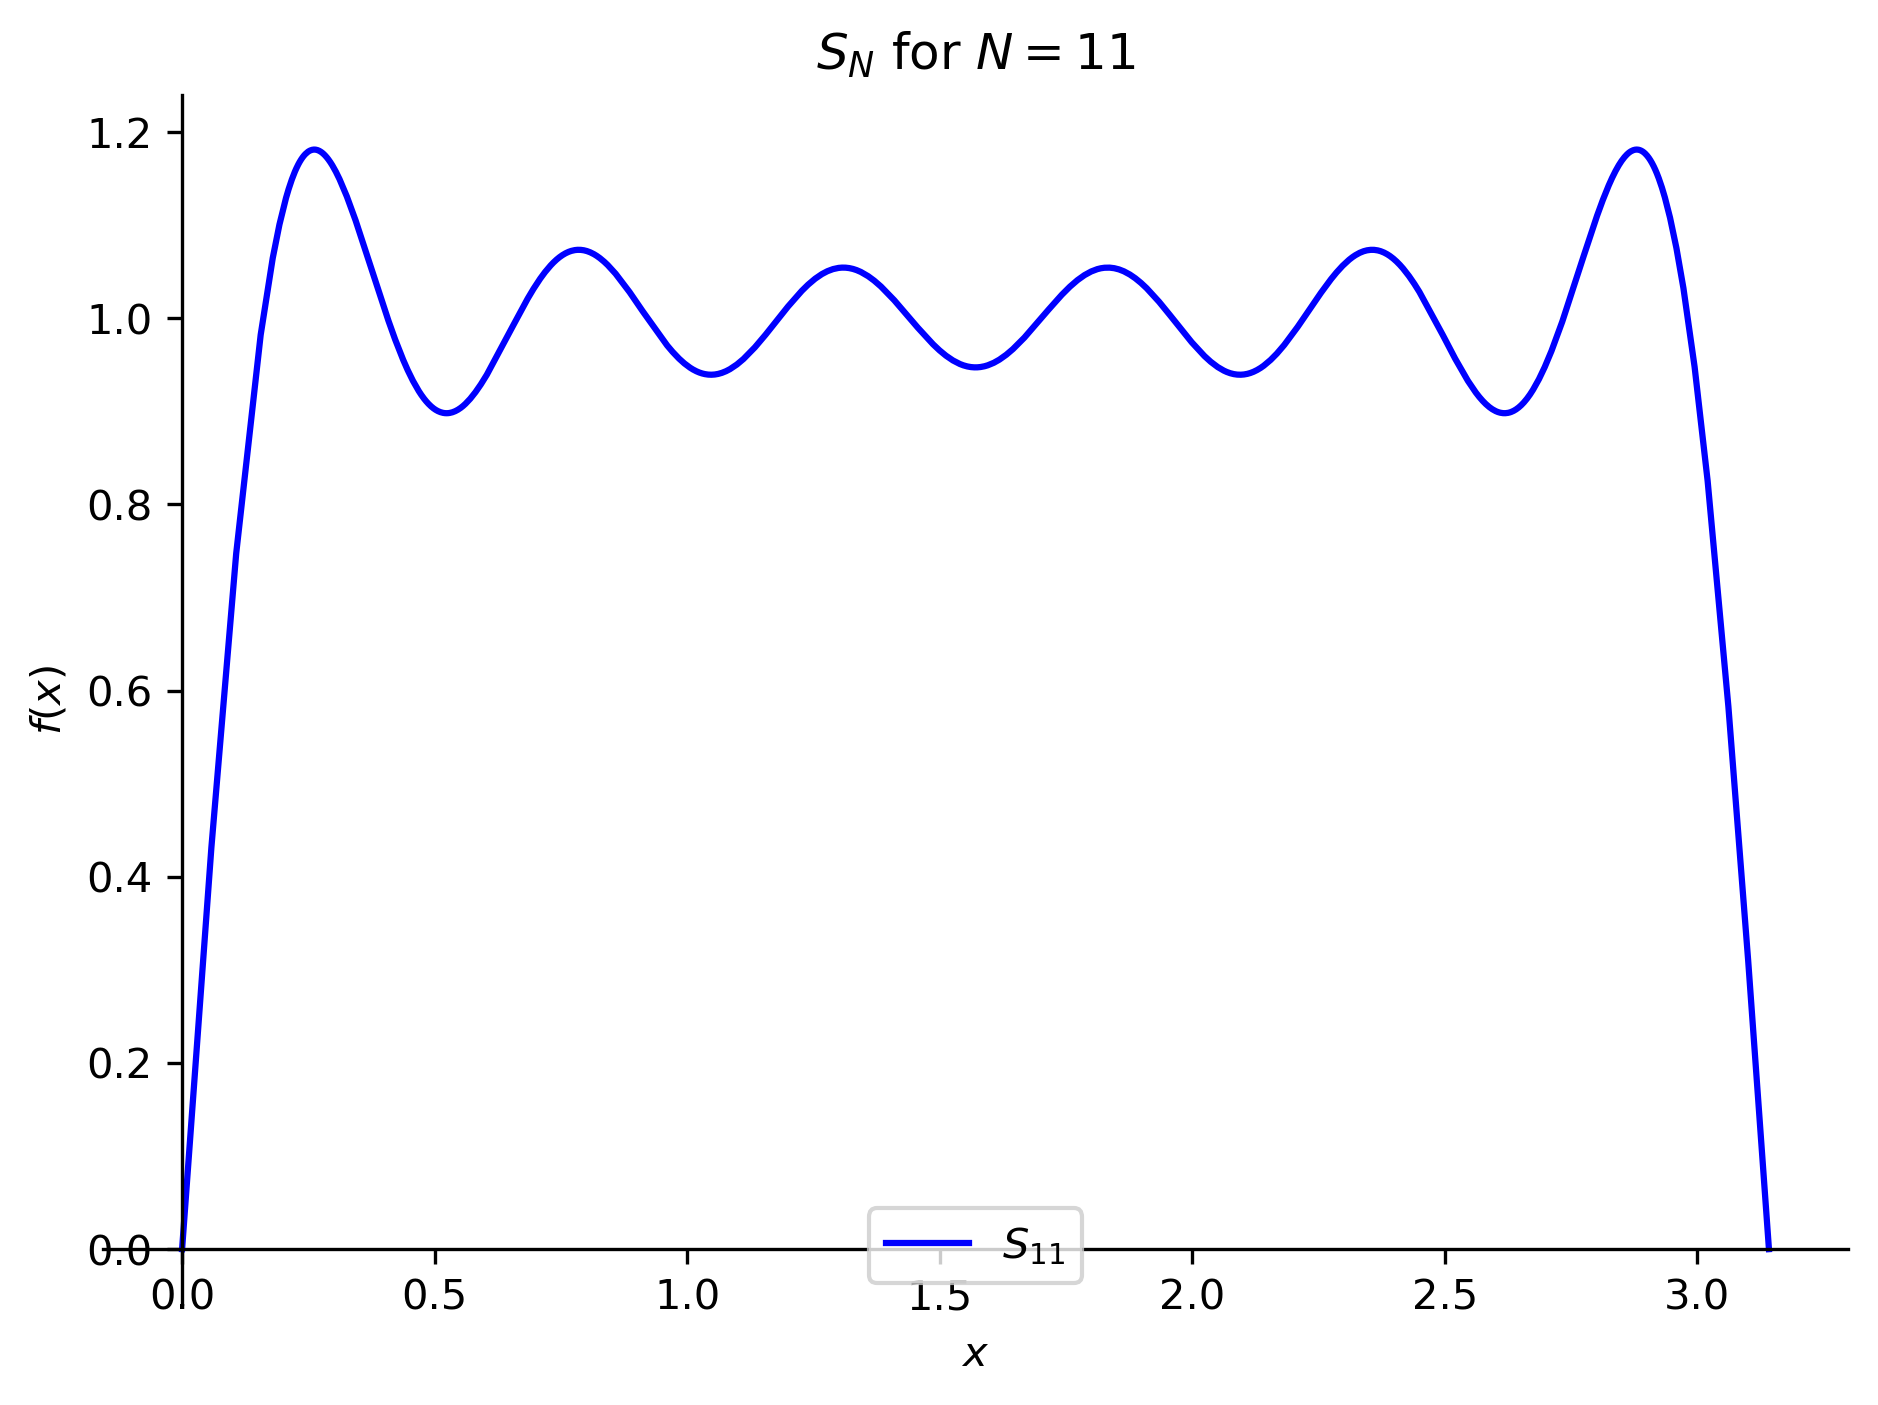
\includegraphics[scale=0.67]{5bs11.png}
    
\end{solution}
\part[1]\starscore14
Let $g(x)=x$ for $0\le x\le\pi$.
Find a formula for $B_n(g)$ valid for every integer $n\ge1$.
\begin{solution}
    \begin{align*}
        B_n(g) &= \frac{2}{\pi} \int^{\pi}_{0} x\sin(nx) \mathrm dx \\
               \intertext{We integrate by parts. Take $u = x$, $\mathrm dv = \sin(nx)$. Then $\mathrm du = \mathrm dx$, $v = -\frac{1}{n}\cos(nx).$}
               &= \frac{2}{\pi} \left(
                    -\frac{1}{n} x \cos(nx) \Big|^{\pi}_{0} + \frac{1}{n} \int^{\pi}_{0}  \cos(nx) \mathrm dx
               \right) \\
               &= \frac{2}{\pi} \left( -\frac{1}{n}\pi \cos(n\pi) \right) \\
               &= -\frac{2}{n}\cos(n\pi)
    \end{align*}

    Again, consider the periodic behaviour of $\cos(n \pi)$. When $n$ is even, $\cos(n\pi) = 1$, when $n$ is odd, $\cos(n\pi) = -1$.

    Therefore,

    \[
        B_n(g) = 
        \begin{cases}
            \begin{aligned}
                -\frac{2}{n} & \text{if } n ~\text{is even} \\
            
                \frac{2}{n} & \text{if } n ~\text{is odd}
            \end{aligned}
        \end{cases}
    \]
\end{solution}
\part[1]\starscore14
Make three plots showing $y=g(x)$ and $y=\wt S_N(x)$ on the same axes, where
\[
\wt S_N(x) = \sum_{n=1}^N B_n(g) \sin(nx).
\]
Use $N=3$ for the first plot, $N=5$ for the second, and $N=11$ for the third.
\begin{solution}

    \centering
    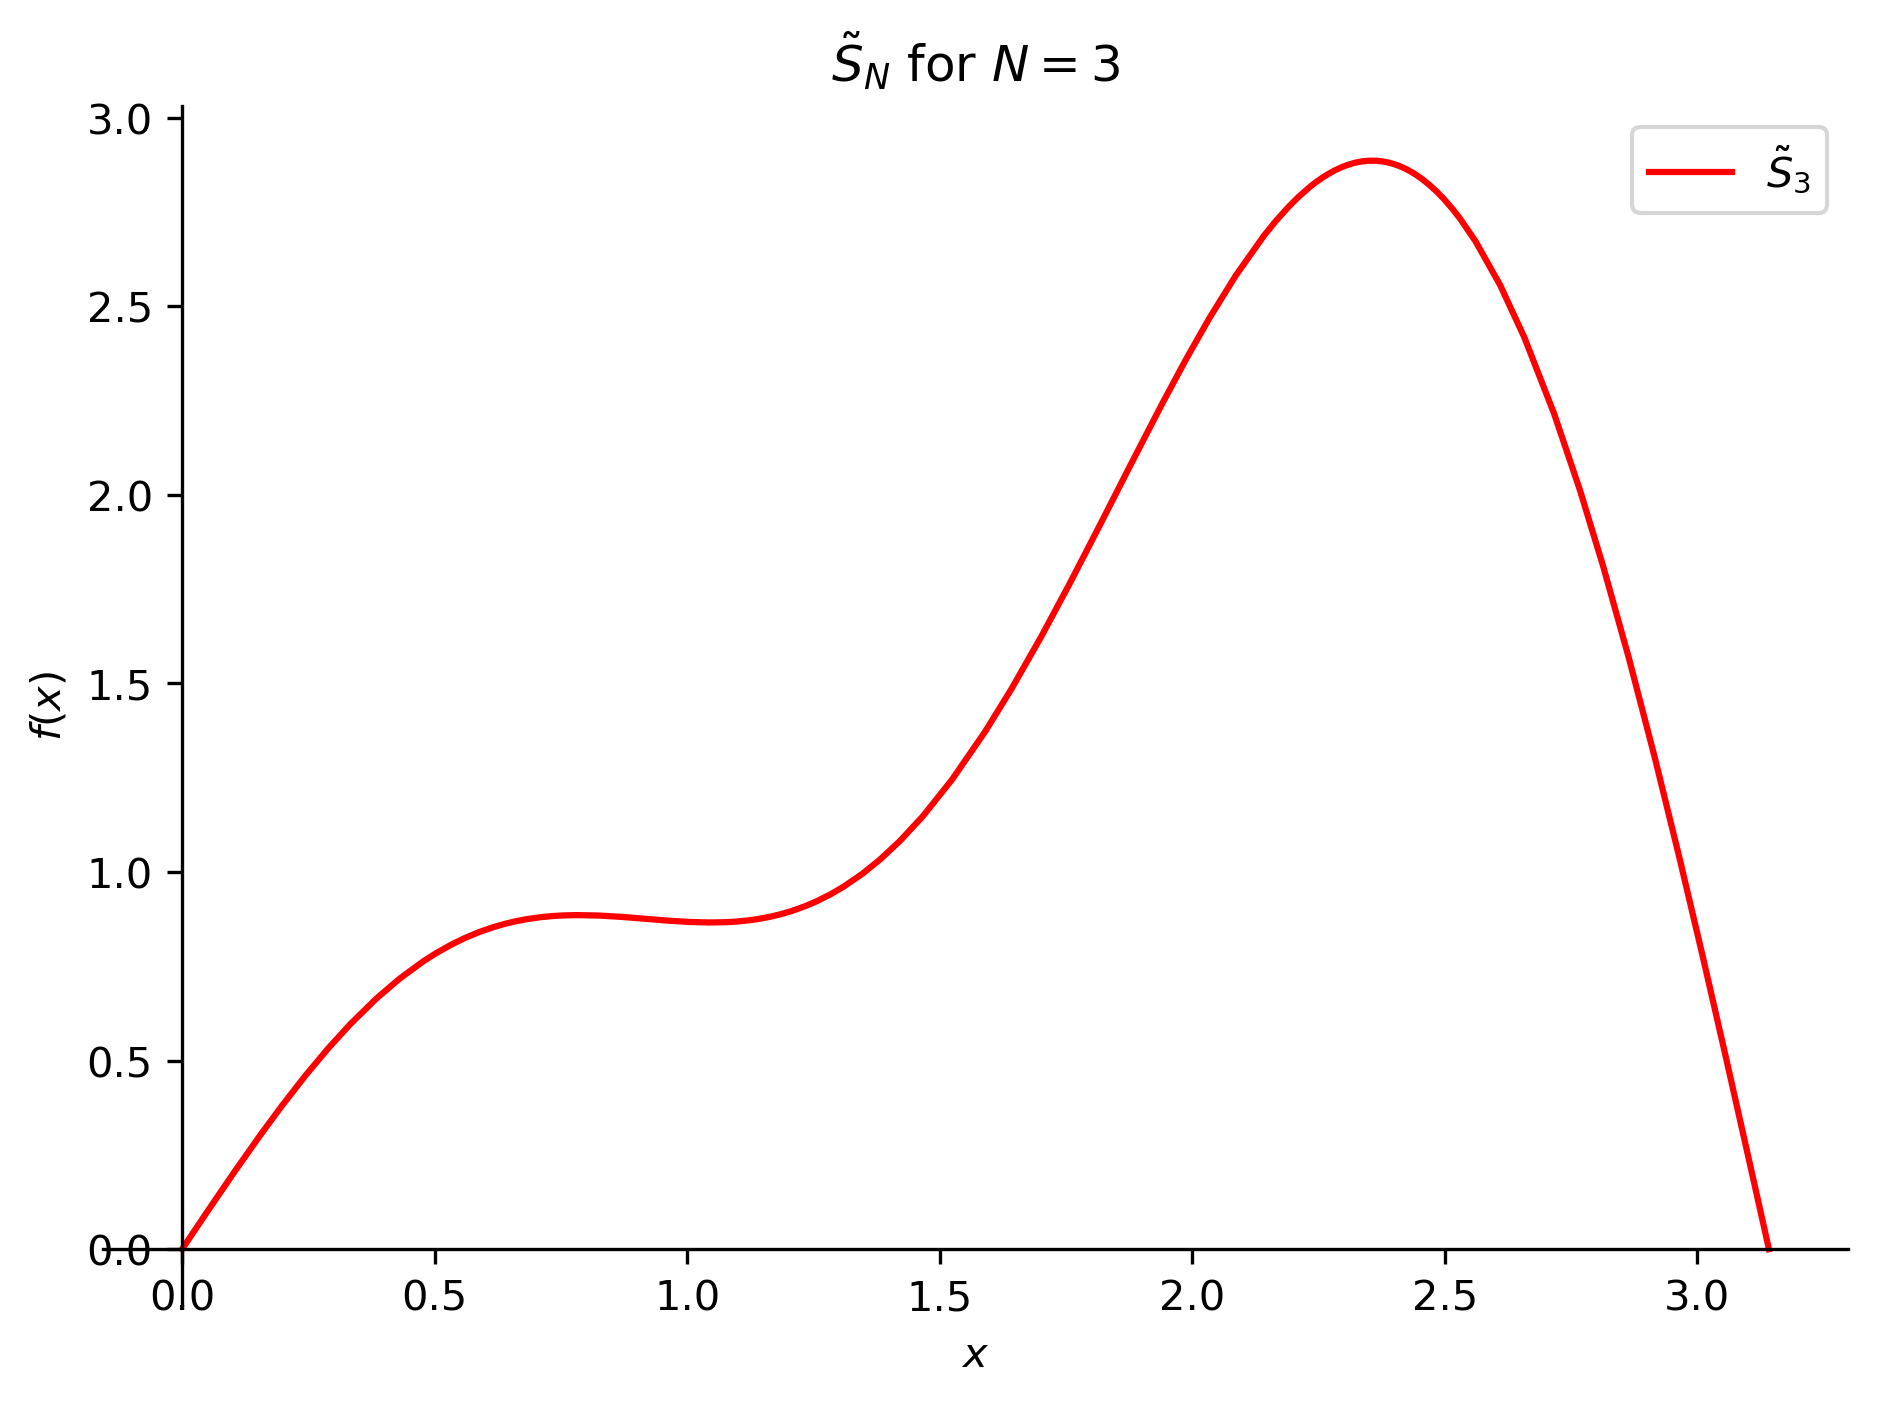
\includegraphics[scale=0.67]{5ds3.png}

    \centering
    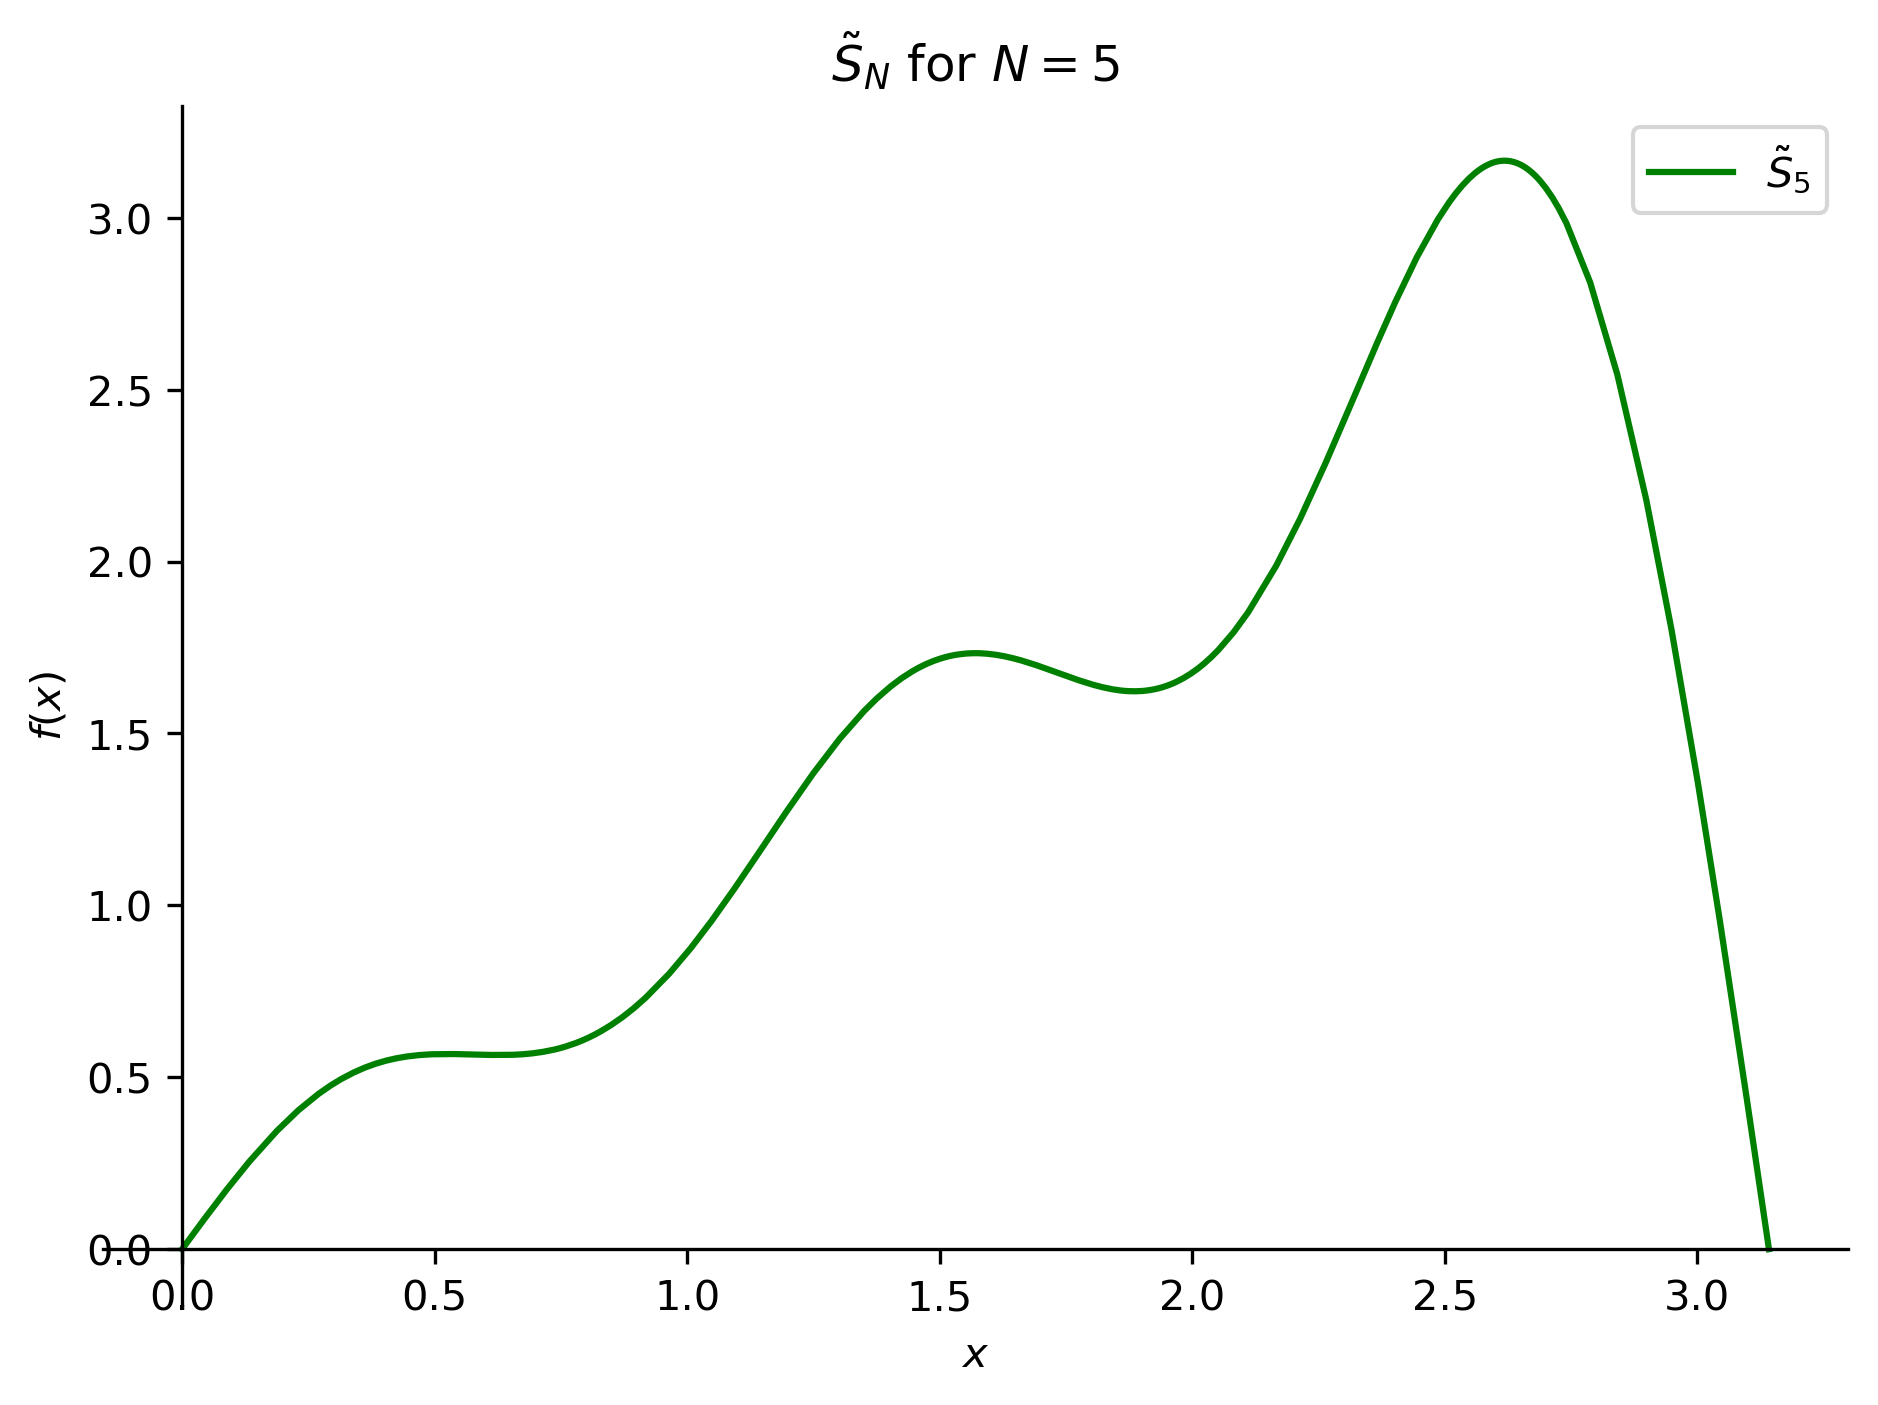
\includegraphics[scale=0.67]{5ds5.png}

    \centering
    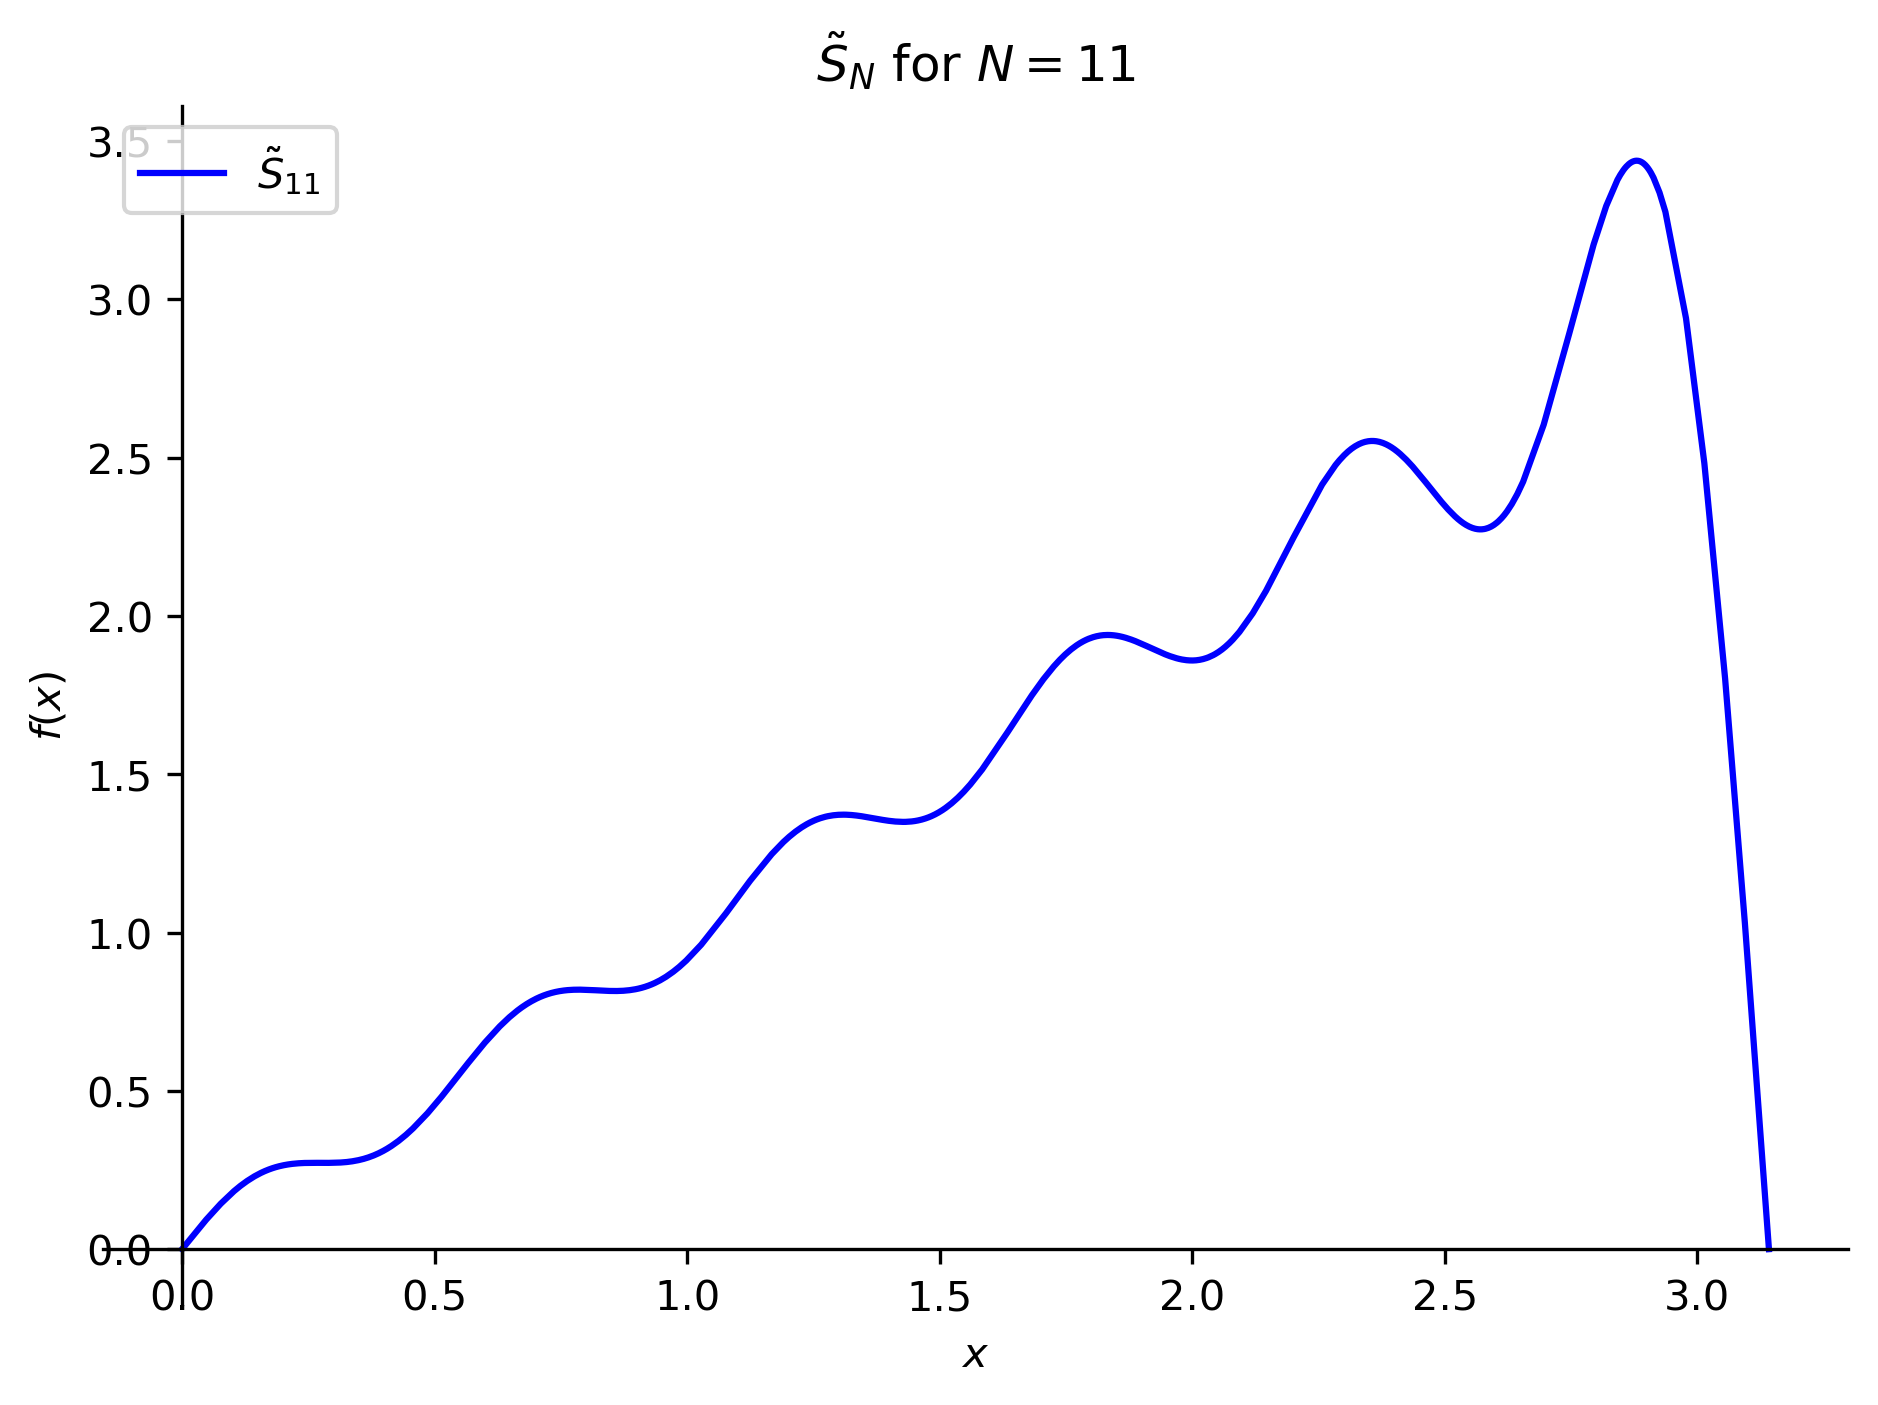
\includegraphics[scale=0.67]{5ds11.png}

\end{solution}
\end{parts}
\end{questions}

\vskip 0pt plus 10fill
\clearpage

\bigbreak\hrule\medskip

\noindent{\textbf{Notes and Comments}}

\begin{itemize}
\item
Question~4 calls for powerful general methods,
which should be capable of handling the tasks in Question~3
with ease.
This makes the simple problem in Question~3 an ideal test-case
for developing a general method.
However, solvers are \emph{not required} to use the same methods
in these two problems.
A simple, direct, no-code solution to Question~3 is fully
acceptable.
\end{itemize}

\noindent{\textbf{Credits}}

\begin{itemize}
\item
The plots shown on the question sheet were made with Desmos.

\end{itemize}

\end{document}
